\chapter{List of papers}
\chapter{Introduction}
The broad topic of this thesis graph based reference genomes, and specifically of mapping and peak calling on such references.
The introduction here is meant to provide an introduction to the topic as well as a coherent brief of the content of the provided papers.
As is common in bioinformatics, full understanding of the field of graph based references requires at least a rudimentary understanding of the underlying biology, mathematics and informatics. An brief introduction to the specific subtopics 

The first section will be an introduction to two main biological topics, reference genomes and genomic variation,
in order to familiarize the reader with topics in addition to establish a perspective that establishes the benefits of graph based references.
Section 2 introduces the concept of sequence graphs and their interpretation in different settings.
Section 3 describes the mathematical formalism used in this thesis as well as the data structures embodying this formalism.
These sections might be persived as too rigorous and opaque for a brief introduction, but this highlights one of the main drawbacks of graphical models, namely their complexity.
% These concepts were introduced in Paper 1: \emph{Coordinates and intervals in Graph Based Reference Genomes}, and further developed in the subsequent papers.
Section 4 and 5 gets to the main focus of this thesis, covering the topics of read mapping and peak calling on graph based reference genomes.


%%% Local Variables:
%%% mode: latex
%%% TeX-master: "main"
%%% End:

\chapter{Background}
\section{Molecular Biology}
\subsection{DNA}
At the heart of molecular biology is \emph{deoxyribonucleic acid}, DNA.
DNA-molecules consist of pairs of four different \emph{nucleotides} linked together to form a double stranded helix.
The four different nucleotides are often represented by the letters A (\emph{adenin}), C (\emph{cytosin}), T (\emph{thymin}) and G (\emph{guanin}), forming an alphabet of nucleotides $\alphabet_{DNA} = \set{A, C, T, G}$.
Each nucleotide can only be paired with one of the others, such that each base-pair in the helix is either (A-T) or (G-C) or opposite. The DNA in a cell is typically organized into long DNA molecules called \emph{chromosomes}. 

The most important function of DNA is to serve as a template for the synthesis of proteins, which in turn are responsible for a wide range of bio-molecular functions.
This is a two-step process where DNA is first \emph{transcribed} to RNA, molecules similar to DNA but single stranded and with \emph{thymin} replaced by \emph{uracil} (U).
The resulting RNA-sequence can in turn be translated to proteins by mapping triplets of ribonucleotides to amino acids, which are the building blocks of proteins.

Sequences of DNA that are transcribed to RNA that either have a function in themselves, or are in turn translated to proteins, are called \emph{genes}.
Genes constitute only a minor proportion of human DNA.
The remaining DNA can be important due to the biochemical properties of the DNA itself. 


\subsection{Replication and Mutation}
In addition to serving as template for RNA molecules, DNA can also be replicated.
This leads to inheritance both on cellular and organismal level.
In normal cell division, the chromosomes are replicated such that each of the two resulting cells have a copy of the DNA from the original cell.
Furthermore, in sexual reproduction germ line cells are copied and transfers half of the organisms chromosomes to an offspring.

However, this DNA-replication is not always accurate.
Errors can occur leading to a copy of the DNA molecule which is not identical with the original.
Most common are the substitution of a single nucleotide, insertion of a small DNA sequence, or deletion of a small subsequence.
Such errors lead to difference between cells within an organism, or difference between individuals.

Difference in the DNA-sequence between two individuals can lead to a change in the transcribed RNA sequence and further in the sequence, and thereby the form and function, of the expressed protein.
It can also lead to less drastic changes such as changes in the RNA-structure or the shape of the DNA molecule itself.
In this way genomic variation can determine differences between specimens of the same species and also differences between the species themselves.

\subsection{Epigenomics}
Difference in DNA-sequence can explain phenotypic
% \TODO{explain geno/pheno}
difference between individuals, but fails to explain the difference between the different cells within an organism.
Within an organism, the cells contain mostly the same DNA-sequences, but exhibit vastly different phenotypes.

The reason for this difference is mostly attributed to differences in expression levels of genes.
Much attention has been devoted in recent years to the mechanisms determining gene expression levels.
Two high-level consortia, ENCODE~\cite{encode} and Roadmap Epigenomics~\cite{roadmap}, have systematically conducted experiments geared towards understanding some of these factors, including: 3D-configuration of the chromosomes, accessiblity of the DNA in different regions, transcription factor binding sites, and methylation patterns across the genome.
Among these, this thesis is concentrated on transcription factor binding sites.
% , but for an introduction to epigenomics as a whole see~\ref{epigenomics}.

Transcription factors are proteins that bind to DNA, with an affinity for certain DNA-sequences.
These proteins signal to other proteins that a gene in their vicinity should be transcribed, thus affecting expression levels of genes.
As such, the presence or absence of transcription factors binding to a binding site can affect the phenotype of a cell.
Also, since the binding of transcription factors is dependent on the DNA-sequence, a mutation in the DNA-sequence in a binding site can affect the binding of the protein and thus the expression of a nearby gene. 

%%% Local Variables:
%%% mode: latex
%%% TeX-master: "main"
%%% End:

\section{Sequencing}
\section{Reference Genomes}
ENCODE data, og gen lister.
The fact that the sequence of nucleotides in the DNA has direct links to biological function has made determining such sequences as well as possible an important goal in molecular biology.
The process of determining the sequence of nucleotides is referred to as DNA-\emph{sequencing}.
The first widely used method for DNA-sequencing was Sanger Sequencing~\cite{sanger}, developed in 1976.
The throughput from Sanger sequencing is pretty low since it requires measuring the weight of many nucleotides.
In the early 2000s, several technologies were developed that were able to parallelize the process of sequencing and thus increased the throughput.
Among these technologies, collectively called Next-Generation Sequencing (NGS), Illumina dye sequencing is the most commonly used, and will be described here.

\subsection{Illumina Dye Sequencing}
Illumina dye sequencing uses sequencing by synthesis, which is the same base methodology as Sanger sequencing.
This method uses the property that given a single strand of DNA and the presence of DNA polymerase, nucleotides will sequentially bind to the strand according to the complementary pairings (A-T) and (C-G).
This usually happens so fast that it is difficult to measure any point in this process.
However, nucleotides can be adapted so that the synthesis is terminated after including the adapted nucleotide (chain termination).
Sanger sequencing uses this by combining a small amount of adapted nucleotides with a larger amount of normal nucleotides, and then using this combined set for DNA synthesis.
Illumina sequencing evolves this concept by also being able to reverse these adaptions so that synthesis can continue~\cite{reversiblechain}. Thus it can step by step synthesize one adapted nucleotide to the single DNA-strand, find out which nucleotide was included, then reverse the adaption and synthesize a new adapted nucleotide(see Figure~\ref{fig:illumina}).
\begin{figure}
  \tikzpicture
    \matrix (m) [matrix of math nodes, align=center, row sep=0.2em, column sep=0.5em, minimum width=1em, minimum height=1.5em]{
A & \dT  &A & T   &A & T   &A & T   \\
C &      &C & \dG &C & G   &C & G   \\
C &      &C &     &C & \dG &C & G   \\
T &      &T &     &T &     &T & \dA \\
G &      &G &     &G &     &G &     \\
};
\draw (m-1-1) -- (m-2-1) -- (m-3-1) -- (m-4-1) -- (m-5-1);
\draw[dotted] (m-1-1) -- (m-1-2);
\draw (m-1-3) -- (m-2-3) -- (m-3-3) -- (m-4-3) -- (m-5-3);
\draw[dotted] (m-1-3) -- (m-1-4);
\draw[dotted] (m-2-3) -- (m-2-4);
\draw (m-1-5) -- (m-2-5) -- (m-3-5) -- (m-4-5) -- (m-5-5);
\draw[dotted] (m-1-5) -- (m-1-6);
\draw[dotted] (m-2-5) -- (m-2-6);
\draw[dotted] (m-3-5) -- (m-3-6);
\draw (m-1-7) -- (m-2-7) -- (m-3-7) -- (m-4-7) -- (m-5-7);
\draw[dotted] (m-1-7) -- (m-1-8);
\draw[dotted] (m-2-7) -- (m-2-8);
\draw[dotted] (m-3-7) -- (m-3-8);

  \endtikzpicture
  \caption{
    Sequencing of one DNA-chain in Illumina sequencing.
    For each step, an adapted nucleotide is added with a phosphorescent color, a picture is taken - capturing the color, and the adaption is reversed allowing for the next nucleotide to be bound.
    Each nucleotide (A, C, G, T) has a different color, so the sequence of colors in the images taken can be used to determine the sequence of nucleotides.}
  \label{fig:illumina}
\end{figure}

The big breakthrough for this sequencing technology was that it could be performed massively in parallel and thereby generate much more sequencing data.
The downside is that while Sanger sequencing could yield up to 700 base pairs long sequences, Illumina sequencing typically yields shorter reads (30-300 base pairs).
This massive amount of relatively short reads is able to give great insights into biology by mapping them to reference genomes.
Reference genomes are covered in Section~\ref{sec:refgenomes}, and the mapping process is covered in Section~\ref{sec:mapping}.

The main error source of Illumina sequencing is that a non-adapted nucleotide can get included in one of the steps, whereupon it is possible for a new nucleotide to get included without the previous one being captured.
To alleviate this, and to obtain a stronger signal, Illumina performs the sequencing steps concurrently on many identical DNA templates. Even so, the number of out-of-sync strands grows with the length of the sequence and puts a practical limit on how many base pairs can be read with certainty.

Depending on which input DNA is provided, this technology can be used to answer a range of biological questions.
One can input unfiltered DNA for sequencing and use the resulting reads to deduce as much of the whole genomic sequence as possible. One can also filter the DNA to contain mostly fragments from protein coding parts of the genome, in order to more efficiently find the DNA-sequence of these regions, from which variations can cause differences in protein structure and function.

In addition to deducing the DNA-sequence of a sample, NGS can also be used to deduce where in the genome biochemical processes occur, for instance the binding of proteins to the genomes. Of importance to this thesis are experiments used to find binding sites for transcription factors, described below. For a more thorough introduction to the methods and applications of NGS, see~\cite{ngs}.

\subsection{ChIP-seq}
\emph{Ch}romatin \emph{I}mmuno\emph{p}resipitation  followed by \emph{seq}uencing (ChIP-seq) is a sequencing experiment that does not aim to determine the genetic variation of the sample, but rather to give insight into where a protein of interest binds to the DNA.

In order to do this, the binding of the protein to DNA is strengthened in order to keep the bindings after the DNA is cut into fragments.
Antibodies for the protein of interest are then used to retrieve DNA-fragments with the protein attached.
These DNA-fragments can then be sequenced, yielding reads that tend to come from the vicinity of a binding site (Figure~\ref{fig:chipseq}). The process of analyzing these reads is covered in Section~\ref{sec:peakcalling}.
\begin{figure}
  \centering
\begin{subfigure}{\textwidth}
  \begin{tikzpicture}[decoration={coil},
dna/.style={decorate, thick, decoration={aspect=0, segment length=1.0cm}},
protein/.style={ellipse, draw=white, minimum width=1cm, minimum height=1cm}]
 
%DNA
\draw[dna, decoration={amplitude=.15cm}] (.0,0) -- (11,0);
\draw[dna, decoration={amplitude=-.15cm}] (0,0) -- (11,0);
\node at (0,0.5) {DNA};
 
%Gene
 \node [rounded corners, fill=green!50, thick, inner xsep=30pt] at (8,0) (box){Gene X};
 \node [protein, minimum height=.75cm,fill=blue!30] at (3,0.5) {CTCF};
\node at (3.5, -0.5) {Transcription Factor};
\draw (1.5, -0.2) rectangle (4.5, 1); 
\end{tikzpicture}
\end{subfigure}
\begin{subfigure}{\textwidth}
  \begin{tikzpicture}[decoration={coil},
dna/.style={decorate, thick, decoration={aspect=0, segment length=1.0cm}},
protein/.style={ellipse, draw=white, minimum width=1cm, minimum height=1cm}]
\tikzstyle{seq}=[font=\ttfamily]
 
%DNA
\node[seq] at (3,0) {ACGTTCGTATATCGTAGCTACTCGAGCTGTAGTTTGATAGATAT};
%Gene
\node [protein, minimum height=.75cm,fill=blue!30] at (3,0.5) {CTCF};
\end{tikzpicture}
\caption{Transcription factor binding to DNA, regulating the expression of Gene X}
\end{subfigure}
\begin{subfigure}{\textwidth}
  \begin{tikzpicture}[decoration={coil},
dna/.style={decorate, thick, decoration={aspect=0, segment length=1.0cm}},
protein/.style={ellipse, draw=white, minimum width=1cm, minimum height=1cm}]
seq/.style={font=\ttfamily}
\tikzstyle{seq}=[font=\ttfamily]
\def\fy{0.4}
% DNA
\node[seq] at (3, 0*\fy) (c1) {ACGTTCGTATATCGTAGCTACTCGAGCTGTAGTTTGATAGATAT};
\node[seq] at (3,-1*\fy) (c2) {ACGTTCGTATATCGTAGCTACTCG....................};
\node[seq] at (3,-2*\fy) (c3) {.......TATATCGTAGCTACTCGAGCTGTA.............};
\node[seq] at (3,-3*\fy) (c4) {...........TCGTAGCTACTCGAGCTGTAGTTT.........};
\node[seq] at (3,-4*\fy) (c5) {..GTTCGTATATCGTAGCTACTCGAG..................};
\node[seq] at (3,-5*\fy) {...TTCGTATATCGTAGCTACTCGAGC.................};
\node[seq] at (3,-6*\fy) {.................CTACTCGAGCTGTAGTTTGATAGA...};
\node[seq] at (3,-7*\fy) {...................ACTCGAGCTGTAGTTTGATAGATA.};
\node[seq] at (3,-8*\fy) {.............GTAGCTACTCGAGCTGTAGTTTGA.......};

\node[left=of c1] {Cell1: };
\node[left=of c2] {Cell2: };
\node[left=of c3] {Cell3: };

%Gene
\node [protein, minimum height=.75cm,fill=blue!30] at (3,0.5) {CTCF};
%0, 7, 11, 2, 3, 17, 19, 13
% 0, 2, 3, 7, 11, 13, 17, 19
\end{tikzpicture}
\caption{DNA Fragments obtained from ChIP different cells}
\end{subfigure}
\begin{subfigure}{\textwidth}
  \begin{tikzpicture}[decoration={coil},
dna/.style={decorate, thick, decoration={aspect=0, segment length=1.0cm}},
protein/.style={ellipse, draw=white, minimum width=1cm, minimum height=1cm}]
seq/.style={font=\ttfamily}
\tikzstyle{seq}=[font=\ttfamily]
\def\fy{0.4}
\node [protein, minimum height=.75cm,fill=blue!30] at (3,0.5) {CTCF};

% DNA
\node[seq] at (3, 0*\fy) {ACGTTCGTATATCGTAGCTACTCGAGCTGTAGTTTGATAGATAT};
\node[seq] at (3,-1*\fy) {\textcolor{red}{ACGTTCGTAT}ATCGTAGCTACTCG....................};
\node[seq] at (3,-2*\fy) {.......TATATCGTAGCTAC\textcolor{red}{TCGAGCTGTA}.............};
\node[seq] at (3,-3*\fy) {...........\textcolor{red}{TCGTAGCTAC}TCGAGCTGTAGTTT.........};
\node[seq] at (3,-4*\fy) {..\textcolor{red}{GTTCGTATAT}CGTAGCTACTCGAG..................};
\node[seq] at (3,-5*\fy) {...TTCGTATATCGTAG\textcolor{red}{CTACTCGAGC}.................};
\node[seq] at (3,-6*\fy) {.................\textcolor{red}{CTACTCGAGC}TGTAGTTTGATAGA...};
\node[seq] at (3,-7*\fy) {...................ACTCGAGCTGTAGT\textcolor{red}{TTGATAGATA}.};
\node[seq] at (3,-8*\fy) {.............GTAGCTACTCGAGC\textcolor{red}{TGTAGTTTGA}.......};
% Gene
\draw[->] (3, -8.5*\fy) -- (3, -9.5*\fy);
\node[seq] at (3, -10*\fy) {ACGTTCGTAT, TACAGCTCGA, TCGTAGCTAC, GTTCGTATAT};
\node[seq] at (3, -11*\fy) {GCTCGAGTAG , CTACTCGAGC, TATCTATCAA, TCAAACTACA};
\end{tikzpicture}
\caption{One end of each fragment is sequenced}
\end{subfigure}

%%% Local Variables:
%%% mode: latex
%%% TeX-master: "sequencing.tex"
%%% End:

\caption{
  Figure showing the main steps of a CHiP-seq experiment. a) A protein of interest (CTCF) binds to the DNA; b) the DNA is cut up into fragments, from which the ones with proteins bound to it are kept; c) these fragments are then sequenced, yielding reads that are from the vicinity of protein binding sites.}
\label{fig:chipseq}
\end{figure}
\subsection{Third Generation Sequencing}
New technologies are continuously being developed, and a set of more recent technologies allows for sequencing of long DNA-molecules.
This does however come at the price of much higher error rates than Illumina sequencing.
Most notable is Oxford Nanopore~\cite{nanopore}, passing DNA-molecules through a molecule which emits a different electric current for each type of nucleotide, and PacBio~\cite{pacbio}, using  nucleotide-dependent light waves emitted continuously while synthesizing.
These techniques offer possibilities for answering biological questions where short read lengths are insufficient, but also new computational challenges for dealing with the high error rates and long read lengths.

%%% Local Variables:
%%% mode: latex
%%% TeX-master: "main"
%%% End:

\section{Mathematical Framework}
The following sections introduces some notation needed for the next chapters. This notation will mainly follow a simplification of the notation used in~\cite{gcsa1}.
\subsection{Sequences}
Sequences are important in this thesis as they are the means to represent DNA-sequences.
We will here formally work with an alphabet $\alphabet_{DNA} = \set{A, C, G, T}$ and say that a \emph{sequence} of length $n$ over that alphabet is a tuple in the set $\alphabet_{DNA}^n$.
The set of all sequences of any length over $\alphabet_{DNA} = \set{A, C, G, T}$ is  represented by $\alphabet_{DNA}^*$.
The length of a sequence $S \in \alphabet_{DNA}^*$ is notated $\size{S}$.
The $i$th symbol in a sequence $s$ is notated $S[i]$ and a substring of $S$ starting at the $i$th symbol (inclusive) and ending at the $j$th symbol (exclusive) is denoted $S[i:j]$.
A \emph{prefix} of $S$, i.e. a substring of $S$ starting from the first symbol, of length $k$ is denoted $S[:k]$, while a \emph{suffix} of $S$ starting at the $k$th symbol is denoted $S[k:]$.
A \emph{kmer} of a sequence $S$ is any substring of $S$ of length $k$.

An \emph{interval} on a sequenence is a tuple of start and end position $(s, e)$.
For an interval $i_S=(s, e)$, the notation $S[i_S]$ will mean the subsequence between the start and end coordinate $S[s:e]$.

For convenience, a string of length $n$ is sometimes represented as $S[:n]$ to convey the size of the string.
Concatenation of two strings $S, T$ are represented as $S \concat T$, while the concatenation of a symbol $a$ to a string $S$ is denoted $Sa$, and a string to a symbol as $aS$.

For some algorithms a $\#$ symbol is added to the start and/or a $\$$ symbol is added to the end of the string.

\subsection{Graphs}
A graph is a tuple $G=(V, E)$ of vertices and edges, where the edges are pairs of vertices $E \subset V^2$.
We will here deal with directed graphs where we say that edge $(v_1, v_2)$ is an edge from $v_1$ to $v_2$.
A \emph{path} is an alternating sequence of vertices and edges $(v_1, e_1, v_2, e_2,,,e_{n-1}, v_n)$ where $e_i = (v_i, v_{i+1})$.
A \emph{cycle} is a path $(v_1, e_1, v_2, e_2,,,e_{n-1}, v_n)$ where $v_1=v_n$ and $n>1$, i.e. a path that starts and ends at the same vertex.
A \emph{directed acyclic graph} (DAG) is a directed graph in which there are no cycles.
We call the set of all paths starting at $v_s$ and ending at $v_e$ $\paths(v_s, v_e)$.
The \emph{predecessors} of a node $v$ are all nodes with an edge going to $v$, i.e: $\preds(v) = \buildset{w \in V}{(w, v) \in E}$.

\subsection{Sequence Graphs}
We define a \emph{sequence graph} $SG = (V, E, \slabel)$ over an alphabet $\alphabet$ as a graph $(V, E)$ and a label function $\slabel: V \rightarrow \alphabet$ labeling each vertex with a letter from $\alphabet$.
We refer to the label of a path $\slabel((v_1, e_1, v_2,,,e_{n-1}v_n))$ as the concatenation of the labels of its vertices $\slabel(v_1)\concat\slabel(v_2) ... \slabel(v_n)$.
The sequence graphs we look at here will have clearly defined start and end nodes, which will be denoted $v_s$ and $v_e$. If this were not the case, dummy nodes ($\#, \$$) can be inserted to the graph to make the start and end unambiguous.
The \emph{language} recognized by a sequence graph $\lang((G, \slabel))$ is the label of each path going from the start node to the end node, i.e:
\[
  \lang((G, \slabel)) = \buildset{ \slabel(p)}{p \in \paths(v_s, v_e)}
\]
A \emph{graph interval} is a path in the graph, and for a graph interval $i_G$, the notation  $SG[i_G]$ will mean the label of that path, i.e. $\slabel(i_G)$.

%%%Local Variables:
%%% mode: latex
%%% TeX-master: "main"
%%% End:

\section{Alignment}
\subsection{Edit Distance}
An edit distance is a measure of How many mutations are required to convert one sequence into  another. Different edit distance measures exists, varying in the set of allowed mutations. The most common is the \emph{Levenshtein distance}~\cite{levensthein}, allowing single character substitutions, insertions and deletions. 

Finding the edit distance between two sequences, and which set of edits this edit distance corresponds to, is of central importance in bioinformatics since it can give an estimate of how related the two sequences are and which mutations have separated them.
The process of finding these estimates is called \emph{sequence alignment} and is important for this thesis in two respects. Firstly, it is one of the earliest and most intuitive applications of sequence graphs, and secondly it is an important part of \emph{mapping} which will be covered in the next section. 

In the following we will refer to the edit distance between two sequences, $S$ and $T$, as $D(S, T)$, meaning the Levenshtein distance unless specifically mentioned. The concepts discussed are however generalisable to other (weighted) edit distances by small changes.

The set of edits between two sequences can be represented with an \emph{alignment block} where ``-'' symbols are inserted into the sequences to represent indels, (see figure~\ref{fig:needle}.

\subsection{Pairwise Sequence Alignment}
Finding the edit distance between two strings is easy if indels are not considered.
It is merely the process of counting the number of mismatches between them.
Indels introduce a dependency since an insertion at position $i$ affects the pairings of all the symbols after position $i$. The number of meaningful combinations of insertions and deletions grow exponentially with sequence length, so exploring all of them is not a viable solution even for short sequences.
The problem is however tractable since the best alignment of two sequences $S[:m], T[:n]$ is either the best alignment of $S[:m-1], T[:n]$ with an insertion at the end, or of $S[:m], T[:n-1]$ with a deletion at the end, or of $T[:n-1], T[:m-1]$ with a match or substitution at the end. 
Letting $d_{i,j} = D(S[:i], T[:j])$ and $m_{i,j}$ be zero if $S[i]=T[j]$ else $1$, we can write this as the recurrence relation:
\begin{align*}
  d_{k,l} = min\begin{cases}
  &d_{k-1,l-1}+m_{k-1, l-1}\quad \text{(match/substitution)}\\
  &d_{k-1,l}+1 \quad \text{(insertion)}\\
  &d_{k, l-1}+1 \quad \text{(deletion)}\\
\end{cases}
\end{align*}
The fact that the edit distance to a empty string is just the sequence length gives $d_{k, 0}=k,\,d_{0,l}=l$.
The Needleman-Wunch algorithm uses dynamic programming to calculate the matrix of edit distances $d_{kl}$, where $d_{mn}$ is the edit distance between $S$ and $T$. In order to find the specific edits, a backtracking algorithm is used that starts at the $(i, j) = (m, n)$ corner and finds out which of the possible predecessors $(i-1, j), (i-1, j-1), (i, j-1)$ contributed to the $(i, j)$ edit distance. Then repeating this until the $(0, 0)$ corner is reached. Each of these steps correspond to a column in the alignment block. Figure~\ref{fig:needle} details the Needleman Wucnch algorithm.
\begin{figure}
  \begin{tikzpicture}
    \matrix (m) [matrix of math nodes, align=right, row sep=0.1em,column sep=0.1em, minimum width=1em, minimum height=1em, nodes={align=right}, ]{\textcolor{red}{0} & \textcolor{black!25}{-1} & \textcolor{black!25}{-2} & \textcolor{black!25}{-3} & \textcolor{black!25}{-4} & \textcolor{black!25}{-5} & \textcolor{black!25}{-6}\\ 
\textcolor{black!25}{-1} & \textcolor{red}{0} & \textcolor{black!25}{-1} & \textcolor{black!25}{-2} & \textcolor{black!25}{-3} & \textcolor{black!25}{-4} & \textcolor{black!25}{-5}\\ 
\textcolor{black!25}{-2} & \textcolor{black!25}{-1} & \textcolor{red}{0} & \textcolor{black!25}{-1} & \textcolor{black!25}{-2} & \textcolor{black!25}{-3} & \textcolor{black!25}{-4}\\ 
\textcolor{black!25}{-3} & \textcolor{black!25}{-2} & \textcolor{red}{-1} & \textcolor{black!25}{-1} & \textcolor{black!25}{-2} & \textcolor{black!25}{-2} & \textcolor{black!25}{-3}\\ 
\textcolor{black!25}{-4} & \textcolor{black!25}{-3} & \textcolor{black!25}{-2} & \textcolor{red}{-1} & \textcolor{black!25}{-1} & \textcolor{black!25}{-2} & \textcolor{black!25}{-3}\\ 
\textcolor{black!25}{-5} & \textcolor{black!25}{-4} & \textcolor{black!25}{-3} & \textcolor{black!25}{-2} & \textcolor{red}{-1} & \textcolor{red}{-2} & \textcolor{black!25}{-3}\\ 
\textcolor{black!25}{-6} & \textcolor{black!25}{-5} & \textcolor{black!25}{-4} & \textcolor{black!25}{-3} & \textcolor{black!25}{-2} & \textcolor{black!25}{-2} & \textcolor{red}{-2}\\ 
\textcolor{black!25}{-7} & \textcolor{black!25}{-6} & \textcolor{black!25}{-5} & \textcolor{black!25}{-4} & \textcolor{black!25}{-3} & \textcolor{black!25}{-3} & \textcolor{red}{-3}\\};
\path[-stealth] (m-1-1) edge [draw=none] node [left=0.5em] {A} (m-2-1);
\path[-stealth] (m-2-1) edge [draw=none] node [left=0.5em] {C} (m-3-1);
\path[-stealth] (m-3-1) edge [draw=none] node [left=0.5em] {G} (m-4-1);
\path[-stealth] (m-4-1) edge [draw=none] node [left=0.5em] {T} (m-5-1);
\path[-stealth] (m-5-1) edge [draw=none] node [left=0.5em] {T} (m-6-1);
\path[-stealth] (m-6-1) edge [draw=none] node [left=0.5em] {A} (m-7-1);
\path[-stealth] (m-7-1) edge [draw=none] node [left=0.5em] {C} (m-8-1);
\path[-stealth] (m-1-1) edge [draw=none] node [above=0.5em] {A} (m-1-2);
\path[-stealth] (m-1-2) edge [draw=none] node [above=0.5em] {C} (m-1-3);
\path[-stealth] (m-1-3) edge [draw=none] node [above=0.5em] {T} (m-1-4);
\path[-stealth] (m-1-4) edge [draw=none] node [above=0.5em] {T} (m-1-5);
\path[-stealth] (m-1-5) edge [draw=none] node [above=0.5em] {G} (m-1-6);
\path[-stealth] (m-1-6) edge [draw=none] node [above=0.5em] {A} (m-1-7);
\path[-stealth] (m-8-7) edge[color=red] (m-7-7);
\path[-stealth] (m-7-7) edge[color=red] (m-6-6);
\path[-stealth] (m-6-6) edge[color=red] (m-6-5);
\path[-stealth] (m-6-5) edge[color=red] (m-5-4);
\path[-stealth] (m-5-4) edge[color=red] (m-4-3);
\path[-stealth] (m-4-3) edge[color=red] (m-3-3);
\path[-stealth] (m-3-3) edge[color=red] (m-2-2);
\path[-stealth] (m-2-2) edge[color=red] (m-1-1);
\matrix (block) [matrix of math nodes, align=right, row sep=0.1em,column sep=0.1em, minimum width=1em, minimum height=1em, nodes={align=right}, below=of m]{A & C & G & T & T & - & A & C\\ 
A & C & - & T & T & G & A & -\\};
\matrix (seqs) [matrix of math nodes, align=right, row sep=0.1em,column sep=0.1em, minimum width=1em, minimum height=1em, nodes={align=right}, above=of m]{A & C & G & T & T & A & C\\ 
A & C & T & T & G & A\\};
  \end{tikzpicture}
  \label{fig:needle}
  \caption{Figure showing the alignment of two sequences using Needleman-Wunch. Each cell in the matrix corresponds to the edit distance between prefixes of $S$ and $T$. The red path shows the backtracking, resulting in an alignment block where each diagonal arrow gives a symbol from both sequences, while horizontal or vertical arrows give an insertion or deletion.}
\end{figure}
This algorithm can be adopted in a number of ways in order to solve related problems.
Notably, by using an affine gap penalty one can reduce the cost of long indels compared to many small indels~\cite{affine}, or one can use positive scores for matches to be able to find subsequences that align well to each other~\cite{smithwaterman}.

An adaption relevant for this thesis, is to find the a subsequence of one sequence $R$ that minimizes the edit distance to another $Q$. I.e find $\min_{k, l}(D(R[k, l], Q)$.
This can be done by changing just the initial conditions of the Needleman-Wunch algorithm, to remove the cost of gaps at the beginning and end of $R$. We set $d_{k0} = 0$ and start the backtracking algorithm at $(m, l)$ where $j=arg min_i d_{mi}$. Figure\ref{fig:needlmanmap} shows an example of this algorithm.
\begin{figure}
  \begin{tikzpicture}
    \matrix (m) [matrix of math nodes, align=right, row sep=0.1em,column sep=0.1em, minimum width=1em, minimum height=1em, nodes={align=right}, ]{\textcolor{black!25}{0} & \textcolor{black!25}{-1} & \textcolor{black!25}{-2} & \textcolor{black!25}{-3} & \textcolor{black!25}{-4} & \textcolor{black!25}{-5} & \textcolor{black!25}{-6}\\ 
\textcolor{black!25}{0} & \textcolor{black!25}{-1} & \textcolor{black!25}{-2} & \textcolor{black!25}{-3} & \textcolor{black!25}{-4} & \textcolor{black!25}{-4} & \textcolor{black!25}{-5}\\ 
\textcolor{black!25}{0} & \textcolor{black!25}{-1} & \textcolor{black!25}{-2} & \textcolor{black!25}{-2} & \textcolor{black!25}{-3} & \textcolor{black!25}{-4} & \textcolor{black!25}{-5}\\ 
\textcolor{black!25}{0} & \textcolor{black!25}{-1} & \textcolor{black!25}{-2} & \textcolor{black!25}{-3} & \textcolor{black!25}{-3} & \textcolor{black!25}{-3} & \textcolor{black!25}{-4}\\ 
\textcolor{red}{0} & \textcolor{black!25}{-1} & \textcolor{black!25}{-2} & \textcolor{black!25}{-3} & \textcolor{black!25}{-4} & \textcolor{black!25}{-3} & \textcolor{black!25}{-4}\\ 
\textcolor{black!25}{0} & \textcolor{red}{0} & \textcolor{black!25}{-1} & \textcolor{black!25}{-2} & \textcolor{black!25}{-3} & \textcolor{black!25}{-4} & \textcolor{black!25}{-3}\\ 
\textcolor{black!25}{0} & \textcolor{black!25}{-1} & \textcolor{red}{0} & \textcolor{black!25}{-1} & \textcolor{black!25}{-2} & \textcolor{black!25}{-3} & \textcolor{black!25}{-4}\\ 
\textcolor{black!25}{0} & \textcolor{black!25}{-1} & \textcolor{red}{-1} & \textcolor{black!25}{-1} & \textcolor{black!25}{-2} & \textcolor{black!25}{-2} & \textcolor{black!25}{-3}\\ 
\textcolor{black!25}{0} & \textcolor{black!25}{-1} & \textcolor{black!25}{-2} & \textcolor{red}{-1} & \textcolor{black!25}{-1} & \textcolor{black!25}{-2} & \textcolor{black!25}{-3}\\ 
\textcolor{black!25}{0} & \textcolor{black!25}{-1} & \textcolor{black!25}{-2} & \textcolor{black!25}{-2} & \textcolor{red}{-1} & \textcolor{red}{-2} & \textcolor{black!25}{-3}\\ 
\textcolor{black!25}{0} & \textcolor{black!25}{0} & \textcolor{black!25}{-1} & \textcolor{black!25}{-2} & \textcolor{black!25}{-2} & \textcolor{black!25}{-2} & \textcolor{red}{-2}\\ 
\textcolor{black!25}{0} & \textcolor{black!25}{-1} & \textcolor{black!25}{0} & \textcolor{black!25}{-1} & \textcolor{black!25}{-2} & \textcolor{black!25}{-3} & \textcolor{black!25}{-3}\\ 
\textcolor{black!25}{0} & \textcolor{black!25}{-1} & \textcolor{black!25}{-1} & \textcolor{black!25}{-1} & \textcolor{black!25}{-2} & \textcolor{black!25}{-2} & \textcolor{black!25}{-3}\\ 
\textcolor{black!25}{0} & \textcolor{black!25}{-1} & \textcolor{black!25}{-1} & \textcolor{black!25}{-2} & \textcolor{black!25}{-2} & \textcolor{black!25}{-3} & \textcolor{black!25}{-3}\\ 
\textcolor{black!25}{0} & \textcolor{black!25}{-1} & \textcolor{black!25}{-2} & \textcolor{black!25}{-2} & \textcolor{black!25}{-3} & \textcolor{black!25}{-2} & \textcolor{black!25}{-3}\\ 
\textcolor{black!25}{0} & \textcolor{black!25}{-1} & \textcolor{black!25}{-2} & \textcolor{black!25}{-3} & \textcolor{black!25}{-3} & \textcolor{black!25}{-3} & \textcolor{black!25}{-3}\\ 
\textcolor{black!25}{0} & \textcolor{black!25}{-1} & \textcolor{black!25}{-2} & \textcolor{black!25}{-2} & \textcolor{black!25}{-3} & \textcolor{black!25}{-4} & \textcolor{black!25}{-4}\\};
\path[-stealth] (m-1-1) edge [draw=none] node [left=0.5em] {G} (m-2-1);
\path[-stealth] (m-2-1) edge [draw=none] node [left=0.5em] {T} (m-3-1);
\path[-stealth] (m-3-1) edge [draw=none] node [left=0.5em] {G} (m-4-1);
\path[-stealth] (m-4-1) edge [draw=none] node [left=0.5em] {G} (m-5-1);
\path[-stealth] (m-5-1) edge [draw=none] node [left=0.5em] {A} (m-6-1);
\path[-stealth] (m-6-1) edge [draw=none] node [left=0.5em] {C} (m-7-1);
\path[-stealth] (m-7-1) edge [draw=none] node [left=0.5em] {G} (m-8-1);
\path[-stealth] (m-8-1) edge [draw=none] node [left=0.5em] {T} (m-9-1);
\path[-stealth] (m-9-1) edge [draw=none] node [left=0.5em] {T} (m-10-1);
\path[-stealth] (m-10-1) edge [draw=none] node [left=0.5em] {A} (m-11-1);
\path[-stealth] (m-11-1) edge [draw=none] node [left=0.5em] {C} (m-12-1);
\path[-stealth] (m-12-1) edge [draw=none] node [left=0.5em] {G} (m-13-1);
\path[-stealth] (m-13-1) edge [draw=none] node [left=0.5em] {C} (m-14-1);
\path[-stealth] (m-14-1) edge [draw=none] node [left=0.5em] {G} (m-15-1);
\path[-stealth] (m-15-1) edge [draw=none] node [left=0.5em] {G} (m-16-1);
\path[-stealth] (m-16-1) edge [draw=none] node [left=0.5em] {T} (m-17-1);
\path[-stealth] (m-1-1) edge [draw=none] node [above=0.5em] {A} (m-1-2);
\path[-stealth] (m-1-2) edge [draw=none] node [above=0.5em] {C} (m-1-3);
\path[-stealth] (m-1-3) edge [draw=none] node [above=0.5em] {T} (m-1-4);
\path[-stealth] (m-1-4) edge [draw=none] node [above=0.5em] {T} (m-1-5);
\path[-stealth] (m-1-5) edge [draw=none] node [above=0.5em] {G} (m-1-6);
\path[-stealth] (m-1-6) edge [draw=none] node [above=0.5em] {A} (m-1-7);
\path[-stealth] (m-11-7) edge[color=red] (m-10-6);
\path[-stealth] (m-10-6) edge[color=red] (m-10-5);
\path[-stealth] (m-10-5) edge[color=red] (m-9-4);
\path[-stealth] (m-9-4) edge[color=red] (m-8-3);
\path[-stealth] (m-8-3) edge[color=red] (m-7-3);
\path[-stealth] (m-7-3) edge[color=red] (m-6-2);
\path[-stealth] (m-6-2) edge[color=red] (m-5-1);
\matrix (block) [matrix of math nodes, align=right, row sep=0.1em,column sep=0.1em, minimum width=1em, minimum height=1em, nodes={align=right}, below=of m]{A & C & G & T & T & - & A\\ 
A & C & - & T & T & G & A\\};
\matrix (seqs) [matrix of math nodes, align=right, row sep=0.1em,column sep=0.1em, minimum width=1em, minimum height=1em, nodes={align=right}, above=of m]{G & T & G & G & A & C & G & T & T & A & C & G & C & G & G & T\\ 
A & C & T & T & G & A\\};
  \end{tikzpicture}
  \label{fig:needlemanmap}
  \caption{Figure showing the alignment of a query sequence $Q$ to a reference sequence $R$, 
Each cell in the matrix corresponds to the edit distance between a prefix of $S$ and a subsequence of  $R$. The red path shows the backtracking, starting at the lowest value of the last column, resulting in an alignment block where each diagonal arrow gives a symbol from both sequences, while horizontal or vertical arrows give an insertion or deletion.}
\end{figure}
This algorithm provides three results: the coordinate $k, l$ of the subsequence of $R$ most similar to $Q$, the edit distance from that subsequence to $Q$, and the set of edits contributing to the edit distance. In this way it solves in a exact, but slow way the problem of the next chapter, namely mapping a read $Q$ to a reference genome $R$.

\subsection{Sequence Graph Alignment}
The framework used to align sequences extends naturally to acyclic sequence graphs \cite{hein, poa}. We define the alignment of a sequence $S$ to a sequence graph $G$ as the alignment of $S$ to a sequence $T \in L(G)$ in the language of $G$ which yields the lowest edit distance.
Similarily, the alignment of two sequence graphs $G, H$, is the alignment of a sequence $S \in L(G)$ to a sequence $T \in L(G)$ that yields the lowest edit distance. 

If we let $d_{ij} = \min_{p_g \in \paths(v_0, v_i), p_h \in \paths(w_0, w_k)}(D(\slabel(p_h), \slabel(p_g)))$ we get a recurrence relation:
\begin{align*}
  d_{ij} &= \min_{v_k \in \preds{v_i}, w_l \in \preds{w_l}} d^*(i, j, k, l)\\
  d^*(i, j, k, l) &= \min \begin{cases}
    d_{il} + 1\\
    d_{kj} + 1\\
    d_{kl} + m_{kl}\\
    \end{cases}    
    \\
    m_{ij} &= 1\, \text{if}\, \slabel(v_i) \neq \slabel(w_j)\, \text{else}\, 0\\
\end{align*}
This is the same as for ordinary sequence alignment, except that all predecessor nodes of $v_i$ and $w_k$ have to be considered, not only $i-1$ and $j-1$ as in the linear case. If the graph is acyclic, then all the $d_{ij}$ can be calculated using dynamic programming, without incurring any infinite loops.
\begin{figure}
  \begin{tikzpicture}
    \matrix (m) [matrix of math nodes, align=right, row sep=0.1em,column sep=0.1em, minimum width=1em, minimum height=1em, nodes={align=right}, ]{. & \# & A & C & T & G & G & G\\ 
\# & \textcolor{red}{0} & \textcolor{black!25}{0} & \textcolor{black!25}{-1} & \textcolor{black!25}{-2} & \textcolor{black!25}{-2} & \textcolor{black!25}{-3} & \textcolor{black!25}{-4}\\ 
A & \textcolor{black!25}{0} & \textcolor{red}{0} & \textcolor{black!25}{-1} & \textcolor{black!25}{-1} & \textcolor{black!25}{-2} & \textcolor{black!25}{-3} & \textcolor{black!25}{-3}\\ 
T & \textcolor{black!25}{-1} & \textcolor{black!25}{-1} & \textcolor{black!25}{-1} & \textcolor{red}{0} & \textcolor{black!25}{-1} & \textcolor{black!25}{-2} & \textcolor{black!25}{-2}\\ 
A & \textcolor{black!25}{-2} & \textcolor{black!25}{0} & \textcolor{black!25}{-1} & \textcolor{black!25}{-1} & \textcolor{red}{-1} & \textcolor{black!25}{-2} & \textcolor{black!25}{-2}\\ 
G & \textcolor{black!25}{-2} & \textcolor{black!25}{-1} & \textcolor{black!25}{-1} & \textcolor{black!25}{-1} & \textcolor{black!25}{-1} & \textcolor{black!25}{-1} & \textcolor{red}{-1}\\};
\path [->] (m-2-1) edge node {} (m-3-1);
\path [->] (m-3-1) edge node {} (m-4-1);
\path [->] (m-3-1) edge[bend right=60] node {} (m-5-1);
\path [->] (m-4-1) edge node {} (m-5-1);
\path [->] (m-5-1) edge node {} (m-6-1);
\path [->] (m-1-2) edge node {} (m-1-3);
\path [->] (m-1-3) edge node {} (m-1-4);
\path [->] (m-1-3) edge[bend left=60] node {} (m-1-5);
\path [->] (m-1-4) edge[bend left=60] node {} (m-1-6);
\path [->] (m-1-5) edge node {} (m-1-6);
\path [->] (m-1-6) edge node {} (m-1-7);
\path [->] (m-1-6) edge[bend left=60] node {} (m-1-8);
\path [->] (m-1-7) edge node {} (m-1-8);
\path[-stealth] (m-6-8) edge[color=red] (m-5-6);
\path[-stealth] (m-5-6) edge[color=red] (m-4-5);
\path[-stealth] (m-4-5) edge[color=red] (m-3-3);
\path[-stealth] (m-3-3) edge[color=red] (m-2-2);
\matrix (am) [matrix of math nodes, align=right, row sep=0.1em,column sep=0.1em, minimum width=1em, minimum height=1em, nodes={align=right}, below=of m]{\# & A & T & A & G\\ 
\# & A & T & G & G\\};
  \end{tikzpicture}
  \label{fig:seqgrapha}
  \caption{Figure showing the alignment of two sequence graphs. Marked in red is the path taken during backtracking. The result is the best alignment of a sequence from the language of each sequence graph. This alignment can again be represented as a sequence graph}
\end{figure}

An alignment between two sequences $S, T$ can be represented by a sequence graph in a meaningful manner in that one can construct a sequence graph $AG(S, T)$ from the alignment of the sequences in such a way that 
\[
\forall (R \in L(AG(S, T)))\left[D(S, R)+D(R, T) =  D(S, T\right)]
\].
For an optimal alignment, this means that all sequences recognized by the sequence graph have the property that the sum of the distance to the original sequences is as low as it can be.
These sequences thus represents combinations of $S$ and $T$ that are natural estimates of an ancestor of the two sequences.
Thus aligning a sequence $S$ to an alignment graph $AG(T, R)$  can be seen as aligning $S$ to the best fitting ancestor sequence of $T$ and $R$
Similarily, aligning two alignment graphs can be seen as finding the ancestors of two pairs of sequences that fits best together.\cite{treealign}. This is illustrated in figure~\ref{fig:treealign}.

\begin{figure}
  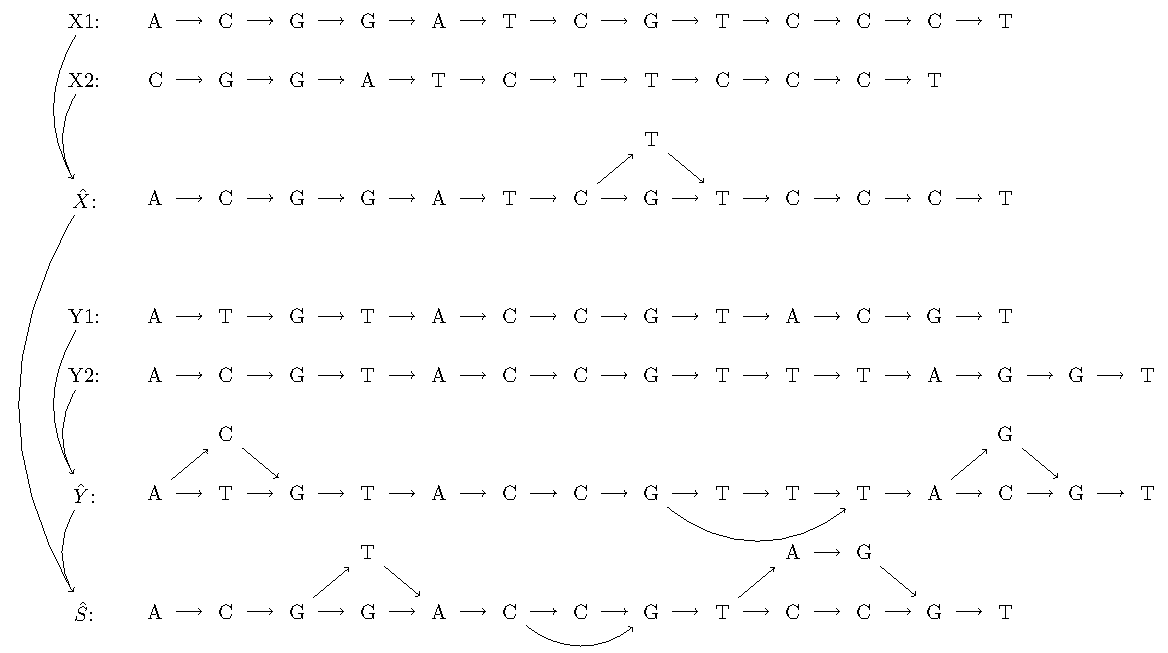
\includegraphics[width=\textwidth,height=\textheight,keepaspectratio]{figures/graph_msa}
  \caption{Iterative sequence graph alignments of four sequences evolved in two generations from \emph{ACGTACGTACGT}.
    The sequences are represented as linear sequence graphs (a) and pairwise alignment is performed on the closest pairs yielding two sequence graphs (b). These two seqence graphs are then aligned to eachother, yielding a sequence graph representing an alignment of the two closest paths in the graphs (c). As seen the original sequence is in the language of the final sequence graph}
  \label{fig:treealign}
\end{figure}

The sequence graph alignment algorithm can also be adapted to find the subsequence of a sequence graph $G_R$ that minimizes the edit distance to a sequence $Q$. This solves the problem of mapping a read to a graph, which will be discussed further in section~\ref{graphmapping}
% \subsection{Large Scale Sequence Alignment}
% In theory, pairwise sequence alignment could be used to find out where a small sequence originates from a large sequence. However, since the Needleman-Wunch alogorithm has complexity $O(n*m)$, it is too computationally demanding to use this directly when dealing with large numbers of sequences and large seqeunces.
% 
%%% Local Variables:
%%% mode: latex
%%% TeX-master: "main"
%%% End:

\section{Mapping}
The alignment methods described in the previous section do not scale well to large sequences.
Aligning a read $Q[:m]$ to a reference genome $R[:N]$ will require computing $mN$ values.
A NGS sequencing experiment typically yields hundreds of thousands of reads of length 50 which need to be located in the human reference genome of length 3 billions.
This would need to calculate $10^{16}$ values, which is intractable even on modern computers. 

This has led to much progress since the dawn of NGS in developing alignment methods that avoid the complexity of the exact dynamic programming methods.
This has been achieved mainly by two \TODO{measures}, creating searchable indexes of the reference genome and using heuristics to limit the search space of possible alignments.

\TODO{In the following is} a brief description of the developments in this field, with focus on the aligner used in this thesis' projects: BWA-mem~\cite{bwamem}.
After this we will look at the methods used  for graph alignment with focus on \emph{vg}~\cite{vg}, which is also central in our work.

\subsection{Linear Mapping}
As in section~\ref{linmap}\TODO{Define this explicitly in alignment}, we define the mapping problem as finding the interval $i_R$ for wich the edit distance $D(R[i_R], Q)$ is smallest, and the alignment $A(R[i_R], Q)$.
\subsubsection{Indexing}
An essential tool for quick alignment is to have a searchable index of the reference genome which is capable of returning sets of interval-pairs from the reference and query sequence for which the reference sequence is identical or near identical to the query sequence.
The indexes used by different tools vary, but can mainly be divided into fixed-length(kmer) indexes~\cite{minimap,,,} and variable-length indexes~\cite{bowtie, bwasw,,,}.
Fixed length indexes typically use hash tables to store the location of a subset of the kmers \TODO{define kmer} in the reference sequence.
Variable length indexes usually use a variation of the \emph{full text minute index} (FM-index)~\cite{fm}, described below.
The main idea covered here is the seed-and-extend paradigm. This idea consists of finding a set of exact matches to the reference sequence, and using these as anchors for using dynamic programming based alignment of the query.
We let $EM(Q, R)$ be the set of all exact matches, represented by the tuples $\buildset{(q, r, l)}{Q[q:q+l]=R[r:r+1]}$.
Since the dynamic programming methods can still be computationally expensive, the goal is to make the seeds\TODO{explain seeds earlier} as small a subset of exact matches as possible, while still making sure that the true alignment covers one of the seeds.

\subsubsection{FM-index}
The FM-index uses a succinct representation of the suffix array~\cite{suffixarray} and Burrows-Wheeler transform~\cite{BWT} of the sequence in order to find exact matches of a query string $S$ in $O(\size{S})$ time (see Figure~\ref{fig:FM}).
Thus if a read has one or more exact matches in the reference sequence it can be found directly using the FM-index.
For inexact matches, it can also be used to find an exact alignment of $Q$ and $R$ in approximately $O(\size{R}^{0.628}\size{Q})$ time~\cite{bwtsw, bwalong}.
Some algorithms also use the FM-index to find exact matches for permutations of the query sequence~\cite{bowtie1, bwashort}, but for longer reads the search space gets too big when allowing for indels.
\begin{figure}
  \tikzpicture
  \matrix (ref) [matrix of math nodes, align=right, row sep=0.2em,column sep=0.2em, minimum width=1em, minimum height=1em, nodes={align=right}, ]{
C & T & A & \textcolor{green}{G} & \textcolor{blue}{C} & \textcolor{red}{T} & \textcolor{green}{G} & C & A & \textcolor{red}{T} & \textcolor{green}{G}\\ 
0 & 1 & 2 & 3 & 4 & 5 & 6 & 7 & 8 & 9 & 10\\};
\node[left=0.2 of ref-1-1] {R:};
\draw (ref-1-7)--(ref-1-6) --(ref-1-5);
\draw (ref-1-11)--(ref-1-10);
\matrix (fm) [matrix of math nodes, align=right, row sep=0.2em,column sep=0.2em, minimum width=1em, minimum height=1em, nodes={align=right}, below=of ref]{
% SA & F & & L & $A_i$ & $C_i$ & $G_i$ & $T_i$ \\
- & \$ & CTAGCTGCAT & $G_0$ & 0 & 0 & 0 & 0\\ 
2 & $A_0$ & GCTGCATG\$C & $T_0$ & 0 & 0 & 1 & 0\\ 
8 & $A_1$ & TG\$CTAGCTG & $C_0$ & 0 & 0 & 1 & 1\\ 
7 & $C_0$ & ATG\$CTAGCT & $G_1$ & 0 & 1 & 1 & 1\\ 
0 & $C_1$ & TAGCTGCATG & \$ & 0 & 1 & 2 & 1\\ 
\textbf{4} & $C_2$ & TGCATG\$CTA & $G_2$ & 0 & 1 & 2 & 1\\ 
10 & $G_0$ & \$CTAGCTGCA & $\textcolor{red}{T_1}$ & 0 & 1 & 3 & 1\\ 
6 & $G_1$ & CATG\$CTAGC & $\textcolor{red}{T_2}$ & 0 & 1 & 3 & 2\\ 
3 & $G_2$ & CTGCATG\$CT & $A_0$ & 0 & 1 & 3 & 3\\ 
1 & $T_0$ & AGCTGCATG\$ & $C_1$ & 1 & 1 & 3 & 3\\ 
9 & $T_1$ & G\$CTAGCTGC & $A_1$ & 1 & 2 & 3 & 3\\ 
5 & $T_2$ & GCATG\$CTAG & $\textcolor{blue}{C_2}$ & 2 & 2 & 3 & 3\\};
\node[above=0.2 of fm-1-1] {SA};
\node[above=0.2 of fm-1-2] {F};
\node[above=0.2 of fm-1-4] {L};
\node[above=0.2 of fm-1-7] {OCC};

\matrix (query) [matrix of math nodes, align=right, row sep=0.1em,column sep=0.2em, minimum width=1em, minimum height=0.5em, nodes={align=right}, below=of fm]{
\textcolor{blue}{C} & \textcolor{red}{T} & \textcolor{green}{G}\\};
\node[color=green, draw, dashed, fit=(fm-7-2) (fm-9-2)] {};
\node[color=red, draw, dashed, fit=(fm-11-2) (fm-12-2)] {};
\node[color=blue, draw, dashed, fit=(fm-6-2)] {};
\draw[dashed, color=red] (fm-7-4) -> (fm-11-2);
\draw[dashed, color=red] (fm-8-4) -> (fm-12-2);
\draw[dashed, color=blue] (fm-12-4) -> (fm-6-2);
\node[left=0.2 of query-1-1] {Q:};
% \node[left=of ref] {R:};
% \node[left=of query] {Q:};


%%% Local Variables:
%%% mode: plain-tex
%%% TeX-master: t
%%% End:

  \endtikzpicture
  \label{fig:FM}
  \caption{Illustration of backward extension using the last-first (LF) property of the FM index.
    The rows represent sorted suffixes of the reference. The SA column holds the indices in the reference sequence for each suffix, the $F$ column holds the first character of each suffix, while the $L$ column holds the preceding character of each suffix. Subscripts give the occurrences of each character in each column. I.e. $T_i$ is the $i$th occurrence of $T$ in that column. Finding the string \emph{CTG} is done by (1) starting with the range of all $G$'s in the F column; (2) finding all $T$'s in this range in the $L$ column; (3) mapping by occurrence number those $T$'s to the F column; (4) mapping the $C$'c in the current range in the L folder by occurrence number. The end result is in this case a single row which represents position $4$ in the reference sequences. 
}
\end{figure}

In order to handle indels in longer reads, the main methodology is to use the FM-index to find exact matches between substrings of the query and reference sequence, called seeds, and then aligning the reads using dynamic programing to intervals surrounding the seed matches on the reference sequence~\cite{bowtie2}, often called the seed-and-extend paradigm.

One way of finding seeds is to find Maximal Exact Matches (MEM)~\cite{longmem, origmem}.
Maximal Exact Matches are Exact Matches that cannot be extended in either direction, ie. 
\[
  MEM(Q, R) = \buildset{(q, r, l) \in EM}{(q, r, l+1) \notin EM \wedge (q-1, r-1, l+1) \notin EM}
\]
BWA-mem furthers this concept to SuperMaximal Exact Matches (SMEM)~\cite{origsmem}.
A SMEM is a MEM where the query interval cannot be extended in either direction and still yields an Exact Match anywhere on the reference~\ref{fig:smem}.
\[
  SMEM(Q, R) = \buildset{(q, r, l) \in EM}{\nexists r^*[(q, r^*, l+1) \notin EM \vee (q-1, r^*-1, l+1) \notin EM}
\]
\begin{figure}
  \tikzpicture
  \matrix (seq) [matrix of math nodes, align=right, row sep=0.5em,column sep=0.5em, minimum width=1em, minimum height=1em, nodes={align=right}, ]{C & T & A & G & C & T & G & C & A & T & G\\ 
G & A & T & C & G & A & C & G & T & A & C\\};
\matrix (q) [matrix of math nodes, align=right, row sep=0.5em,column sep=0.5em, minimum width=1em, minimum height=1em, nodes={align=right}, below=of seq]{T & A & C & T & G & A & T & G\\};
\node[color=red, draw, dashed, rounded corners, fit=(q-1-3) (q-1-5)] {};
\node[color=red, draw, dashed, rounded corners, fit=(seq-1-5) (seq-1-7)] {};
\node[color=green, draw, dashed, rounded corners, fit=(q-1-1) (q-1-2)] {};
\node[color=green, draw, dashed, rounded corners, fit=(seq-1-2) (seq-1-3)] {};
\node[color=green, draw, dashed, rounded corners, fit=(seq-2-2) (seq-2-3)] {};
\node[color=blue, draw, dashed, rounded corners, fit=(q-1-6) (q-1-8)] {};
\node[color=blue, draw, dashed, rounded corners, fit=(seq-1-9) (seq-1-11)] {};
\node[color=blue, draw, dashed, rounded corners, fit=(seq-2-8) (seq-2-10)] {};
  \endtikzpicture
  \label{fig:smem}
  \caption{SMEMs found between query $Q$ and both strands of reference $R$. Note that the MEM $(q, r, l)=(2, 0, 2)$ (CT) is not a SMEM, since it is contained in the SMEM $(q, r, l) = (2, 4, 3)$}
\end{figure}

SMEMS are natural to use as seeds as they cover for each subsequence in $Q$ the longest exact match in $R$.
They are however vulnerable for spurious long matches hiding shorter exact matches.
To account for this BWA-mem allows an option to split long SMEMs into shorter MEMs if they are longer than a certain threshold.
Splitting SMEMs like this increases accuracy, since it increases the number of seeds, but can negatively affect performance. 
In order to find SMEMS, an adaption of the FM index is used, the FMD index, where $FMD(R) = FM(R \concat \bar{R})$.

\subsubsection{Prioritizing and Extending}
The seeds found from the index are next used as seeds for DP based alignment.
$Q$ is then aligned against the left and right side of $(r, r+l)$ for each seed $(q, r, l)$.
Since this is a computationally expensive step, further limiting the set of seeds is advantageous.
BWA-mem does this by \emph{chaining} the seeds.
This is done by grouping approximately collinear, nearby seeds into chains, and removing small chains that overlap with larger chains.
Approximately collinear means that $\abs{(q_1-q_2) -(r_1-r_2)}<w$ for some set threshold $w$.

\subsection{Graph Mapping}
Mapping to a graph based reference is similar to the linear case, except that instead of finding a linear interval, the goal is to find a graph interval $i_r$ such that $D(\slabel(G_R(i_r), Q))$ is minimized. 

% estimating a linear interval $(\hat{s}, \hat{e})$, a graph interval $(\hat{s}, \hat{e}, \hat{v})$ is estimated.
It is however deceptively more complicated. 
Firstly, because the number of subsequences in a sequence graph grows exponentially with the complexity of the graph, and secondly since chaining subsequence-matches is more complicated due to the possible existence of multiple paths between two matches.
\emph{vg}~\cite{vg} has been at the forefront of mapping to a graph reference, showing that it can lead to better mapping accuracy than BWA-mem. 
% But it is still too slow and memory- and disk-consuming for widespread use.
Below is a brief description of the methodology used by \emph{vg}.

\subsubsection{\emph{vg}}
\emph{vg} uses much the same methodology as BWA-mem to align reads.
It uses the GCSA2-index to find SMEMs, uses chain \TODO{filtering to filter} the SMEMs, and uses a graph adaption of Smith-Waterman to extend the seeds.
\emph{vg} is able to align reads to more complicated graph structures than the simple directed sequence graphs considered in this thesis.
For simplicity, the descriptions below will be contained to simple graphs, which entails that the GCSA index described is GCSA1\cite{gcsa1} which is only able to index directed sequence graphs.

\subsubsection{GCSA}
The GCSA-index~\cite{gcsa, gcsa2} is a generalization of the FM-index, where arbitrary-length sequences can be looked up in a sequence graph.
Originally constructed to work on acyclic sequence graphs, GCSA2 extends the functionality to general variation graphs.
For simplicity we will here constrain the discussion to acyclic graphs.

\TODO{clearer GCSA12}
GCSA uses the same concept of $LF$ mapping as the FM-index does. Here the F column holds the label of each node in the graph, sorted by the suffix starting from that node. The L column holds the label of the corresponding node's predecessor nodes. The problem with this setup is that there are many suffixes starting from each node, depending on which path is taken in the graph. To resolve this problem, the graph needs to be expanded so that for each node, all suffixes starting from that node shares a prefix that is not found from any other node in the graph (see Figure~\ref{fig:gcsa} ).

For complicated regions in the graph, this expansion procedure gets too costly, and the GCSA index therefore needs to prune edges in such areas in order to be able to index it. This means that not all possible sequences in the graph gets indexed. Even after pruning, this procedure is costly and makes the GCSA index significantly slower to create, and more memory consuming than the FM-index.

\begin{figure}
  \tikzpicture
  \matrix (seq) [matrix of math nodes, align=right, row sep=0.5em,column sep=0.5em, minimum width=1em, minimum height=1em, nodes={align=right}, ]{G & C & A & C & G\\ 
 &  & T &  & \\};
\draw (seq-1-1) -- (seq-1-2);
\draw (seq-1-1) -- (seq-1-2);
\draw (seq-1-2) -- (seq-1-3);
\draw (seq-1-2) -- (seq-2-3);
\draw (seq-1-3) -- (seq-1-4);
\draw (seq-2-3) -- (seq-1-4);
\draw (seq-1-4) -- (seq-1-5);
\draw (seq-1-4) -- (seq-1-5);

\matrix (seqe) [matrix of math nodes, align=right, row sep=0.5em,column sep=0.5em, minimum width=1em, minimum height=1em, nodes={align=right},right=of seq]{
G & C  & A & C & G\\ 
  & C  & T &   &  \\};
\draw (seqe-1-1) -- (seqe-1-2);
\draw (seqe-1-1) -- (seqe-2-2);
\draw (seqe-1-2) -- (seqe-1-3);
\draw (seqe-2-2) -- (seqe-2-3);
\draw (seqe-1-3) -- (seqe-1-4);
\draw (seqe-2-3) -- (seqe-1-4);
\draw (seqe-1-4) -- (seqe-1-5);
\draw (seqe-1-4) -- (seqe-1-5);
\matrix (gcsa) [matrix of math nodes, align=right, row sep=0.5em,column sep=0.5em, minimum width=1em, minimum height=1em, nodes={align=right},below=of seq]{
SA &  & BWT\\
  & $\$$ & $G_0$ \\
2 & $A_0$ & $C_0$ \\
1 & $C_{0,1}$ & $G_1$ \\
4 & $C_{2}$ & $A_0, \textcolor{red}{T_0}$ \\
6 & $G_{0}$ & $C_1$ \\
0 & $G_{1}$ & $\$$ \\
3 & $T_0$ & $\textcolor{blue}{C_2}$\\
};
\draw[dotted] (gcsa-5-2) -- (gcsa-5-3);
\draw[dotted, color=red] (gcsa-5-3)  -- (gcsa-8-2);
\draw[dotted] (gcsa-8-2) -- (gcsa-8-3);
\draw[dotted, color=blue] (gcsa-8-3) -- (gcsa-5-2);

\matrix (gcsag) [matrix of math nodes, align=right, row sep=0.5em,column sep=0.5em, minimum width=1em, minimum height=1em, nodes={align=right},below=of seqe]{
SA &  & BWT\\
  & $\$$ & $G_0$ \\
2 & $A_0$ & $C_0$ \\
1 & $C_0$ & $G_1$ \\
5 & $C_1$ & $A_0, \textcolor{red}{T_0}$ \\
3  & $C_2$ & $\textcolor{yellow}{G_2}$ \\
7 & $G_{0}$ & $C_1$ \\
\textbf{0} & $G_{1,2}$ & $\$$ \\
4 & $T_0$ & $\textcolor{blue}{C_2}$\\
};
\draw[dotted] (gcsag-5-2) -- (gcsag-5-3);
\draw[dotted, color=red] (gcsag-5-3)  -- (gcsag-9-2);
\draw[dotted] (gcsag-9-2) -- (gcsag-9-3);
\draw[dotted, color=blue] (gcsag-9-3) -- (gcsag-6-2);
\draw[dotted] (gcsag-6-2) -- (gcsag-6-3);
\draw[dotted, color=yellow] (gcsag-6-3) -- (gcsag-8-2);
%\draw[dotted] (gcsa-5-2) -- (gcsa-5-3) -- (gcsa-8-2) -- (gcsa-8-3);\\


\node[above=of seq] {Invalid};
\node[above=of seqe] {Valid};

\node[color=green, draw, dashed, fit=(gcsa-4-2) (gcsa-5-2)] {};
\node[color=red, draw, dashed, fit=(gcsa-8-2)] {};
\node[color=blue, draw, dashed, fit=(gcsa-5-2)] {};

\node[color=green, draw, dashed, fit=(gcsag-4-2) (gcsag-6-2)] {};
\node[color=red, draw, dashed, fit=(gcsag-9-2)] {};
\node[color=blue, draw, dashed, fit=(gcsag-6-2)] {};
\node[color=yellow, draw, dashed, fit=(gcsag-8-2)] {};


\matrix (query) [matrix of math nodes, align=right, row sep=0.1em,column sep=0.2em, minimum width=1em, minimum height=0.5em, nodes={align=right}, below=of gcsa]{
\textcolor{yellow}{G} & \textcolor{blue}{C} & \textcolor{red}{T} & \textcolor{green}{C}\\};
%%% Local Variables:
%%% mode: plain-tex
%%% TeX-master: t
%%% End:

  \endtikzpicture
  \label{fig:gcsa}
  \caption{
    Valid and invalid GCSA index.
    In the first graph, the two edges from $C$ to $A$ and$T$ makes a direct GCSA index impossible due the other $C$ with an edge to a $G$.
    Both $T$ and $G$ needs to point to the same row in the index.
    In the valid example, the $C$ node have been duplicated.
    The bifurcation now happens at an earlier point, and the $GC$ now present is unique so that the the LF mapping is valid.}
\end{figure}

Since the GCSA index provides the same functionality as an FM-index, it can be used to find SMEMs in much the same manner. These SMEMs are in \emph{vg} used as seeds. 

GCSA2 solves the problem in a slightly different way that allows for indexing general variation graphs.
This is based on succinct de-Bruijn graph~\cite{succinctdebruijn} structure which sets a limit to the length of the unique prefixes by allowing for false positive edges to occur in the index.
This means that results from an index lookup needs to be validated by traversing the graph. 

\subsubsection{Filtering and Extending}
\emph{vg} employs a similar method as BWA-mem for filtering out seeds: chaining the seeds and filtering out small chains that overlap bigger chains.
The chaining procedure is however more complicated on a graph, and involves clustering the seeds by position in addition to a Markov Model based method\TODO{cite} to find approximately collinear seeds. 

%%% Local Variables:
%%% mode: latex
%%% TeX-master: "main"
%%% End:

\section{Peak Calling}
Chip-seq is an experiment designed to elucidate where a transcription factor binds. Immunoprecipitation is used to isolate small fragments of DNA which have the transcription factor bound to them.
Ends of these framgents are then sequencesed yielding reads that in general are assumed to be in the vincinity of a binding site. In order to find from this where the transcription factor was bound bioinformatics pipelines are needed.
This is in general consists of mapping the reads to a reference genome, and performing \emph{peak calling} on the coordinates of the mapped reads.
Peak calling is required to estimate from the mapped reads,
only known to tend to be in the vicinity of a binding site, where the binding site is.
The input to peak calling is a set of directed intervals and the output is generally either a set of positions, or a set of undirected intervals that denote the predicted binding sites. 
\[PC: \intervals_G \rightarrow \intervals^+_G\] 
A range of methods for performing peak calling exists~\cite{macs2, SPP, peakcallreview}.
In the following is described the algorithms used by MACS2 and the adaptions to those algorithms used by Graph Peak Caller descirbed in Paper 3 and Paper 4.

\subsection{MACS2}
The input is a set of intervals $\set{(s_k, e_k, d_k)}$. The first step is to count how many extended reads cover each position of the reference genome, where each interval is extended to a length equaling a previously estimated fragment length $f$. I.e for each position $i$ we want to find the count
$$P(i)= \size{\buildset{k}{d_k=1 \wedge s_k \leq i < s_k+f} \cup \buildset{k}{d_k=-1 \wedge e_k-f \leq i < e_k}}$$
  The pileup function $P$ is represented sparsely by a set of indices $\set{s_k}$ and values $\set{v_k}$ such that $$\forall{k}\forall{j\in\set{s_k, s_k+1},,,s_{k+1}}(P(j) = v_k)$$
  the indices and values are found algorithmically as
  \begin{lstlisting}
def count_extended(intervals, f):    
    starts = [s if d==1 else e-f for s, e, d in intervals]
    ends = [e if d==1 else s+f for s, e, d in intervals]
    changes = starts+ends
    args = argsort(changes)
    codes = [1 if arg<=len(starts) else -1 for arg in args]
    s = changes[args]
    v = cumsum(codes)
    return s, v
  \end{lstlisting}
  Which is done in $O(n \log n)$ time. The counts for each position is compared with a background track which represents a local average of reads. This is generated by using a large extension length and dividing the pileup values by the extension size.
  \code{s, v = count_extended(control_intervals, E)/E; v/=E}.
  Assuming that each count $P(i)$ are Poisson distributed as $P_i ~ Poisson(\lambda_i)$, a null hypothesis of $H_0^i: \lambda_i=C(i), H_a^i:\lambda_i>C(i)$ is made for each position and a p-value calcluated: $p_i = P(P_i>=P(i))$ \TODO{too many ps}. Too adjust for multiple testing, a final set of q values is calculated as $q_i = p_iN_i$ where $N_i = \size{\buildset{k\in\set{1, 2,,,\size{G}}}{p_k\leq p_i}}$. The q values are thresholded on a given significance level $\alpha$ so we get $T(i) = q_i\leq \alpha$. 
  \begin{lstlisting}
def get_p_values(pileup, background):
    indices = pileup.indices + background.indices
    indices.sort()
    pileup_values = pileup.values[search_sorted(indices, pileup.indices)]
    background_values = background.values[search_sorted(indices, background.indices)]
    p_values = poisson.sf(pileup_values, background_values)
    return Pileup(indices, p_values)
  \end{lstlisting}
Which is done in $O(n)$ time.
\begin{lstlisting}
def get_q_values(p_values):
    counts = diff(p_values.indices)
    args = argsort(p_values.values)
    values, idxs = unique(p_values, return_index=True)
    N = cumsum(counts[args])[idxs]
    q_values = N*values
    all_q_values = zeros_like(p_values.values)
    all_q_values[idxs] = diff(q_values)
    all_q_values = cumsum(all_q_values)
    restored = zeros_like(all_q_values)
    restored[args] = all_q_values
    return Pileup(p_values.indices, restored)
  \end{lstlisting}
  The thresholded values are obtained simply by \code{Pileup(q_values.indices, q_values.values>alpha)}.

The final peaks are called in two steps from the thresholded values. First, joining peak intervals that are separated by less than the estimated read length, and secondly removing peaks that are shorter than the estimated fragment length $f$. Both steps can be made using the same function.
\begin{lstlisting}
def remove_small(indices, size):
    indices = indices.reshape((-1, 2))
    lengths = indices[:, 1]-indices[:, 0]
    big_enough = lengths>=size
    return indices[big_enough].ravel()

peaks = r_[indices[0], remove_small(indices[1:-1], read_length), indices[-1]]
peaks = remove_small(peaks, fragment_length)
\end{lstlisting}


% 
% 
% 
% 
%  of positions in the graph.
% rd$ by \code{node_offsets[v]+o}. The inverse conversion of a coordinate $i \in \linearcoord$ is done by \code{v=searchsorted(node_offset, i); o = i-node_offsets[v])}
% 
% 
% 
% 
% 
% 
% 
% 
% 
% 
% 
% 
% 
% 
% 
% 
% 
% 
% 
% 
% 
% 
% 
% 
% 
% 
% 
% 
% 
% 
% 
% 
% 
% 
% 
% 
% 
% 
% 
% 
% 
% 
% 
% 
% 
% 
% 
% ̈́onger than the estimated fragment length.


%%% Local Variables:
%%% mode: latex
%%% TeX-master: "main"
%%% End:

\chapter{Summary of Papers}
\chapter{Discussion}
This thesis comprises three projects that investigates different facets of graph based reference genomes.
In this work, and in the work of others, some problems have become clear which relate to the potentially large number of sequences in the language of a sequence graph. Foremost of these are the computational complexity of dealing with this large set of potential sequences, and the large number of sequences that does not exist in any observed individual.

\subsection{Computational Complexity}
The work in paper II and III involved using mapping reads using \emph{vg}.
Although the method used there is in principle very similar to what is used by BWA-mem, the memory requirements and running times are significantly higher.
Graph Peak Caller itself also suffers from requiring more memory and having longer running times than MACS2. 
Although algorithmic and data structural advances might alleviate these problems, some complexities might not be resolvable without turning to further approximations, or changing the interpretation of sequence graphs.
Indeed, Massimo et al showed that the indexing of sequence graphs is a hard problem with theoretical lower bound on complexity~\cite{indexcomplexity}.

When the field of bioinformatics in recent years have been dominated by the sequencing capacity growing faster than Moore's law, it is worth to wonder how much accuracy gains is needed to justify the increase in computational complexity.

\subsection{Invalid Sequences}
Not only computational performance is affected by the large number of sequences in a graphs language.
It can also lead to a large number of sequences that one would not expect to observe in nature.
This is because all combinations of variants are represented in the language, but in nature variants can be highly positively of negatively correlated with each other.
Such sequences makes graph mappers prone to mapping reads to sub sequences in the graph that matches the query string, but is unlikely to be the true origin of the read.
This can lead to a loss of accuracy when mapping, but can also introduce biases in downstream analysis: Regions of the graph with many variants will be able to match many different query sequences and can thus become over represented when mapping reads to a graph.
This potential bias is discussed in briefly in Paper II, where such over represented regions could be interpreted as peaks by the peak caller.
The loss of accuracy in general can be seen in paper II in the relatively poor performance of graph mappers on reads not containing any variants.
The two step approach introduced there can remedy such mapping effects, and it would be interesting in the future to use this approach also when calling ChIP-seq peaks, as this could remove the bias. 

Recent work has introduced indexes for sequence graph that only index substrings that are present in one of the sequences which was used to create the graph~\cite{haplotypeaware}.
This approach has the potential of both reducing the computational complexity, and improve the accuracy of the read mapping.
It will be interesting to see how such approaches perform in the benchmarks from Paper III, and also if they can improve the accuracy of downstream peak calling for ChIP-seq experiments.

\subsection{Conclusion}
In this thesis, the role of reference genomes have been investigated from several angles with a focus on how a change to a graph based representation can affect commonly performed analyses.
As discussed above, a graph based representation carries with it some inherent complexities.
However, these complexities aside, we have shown that a graph based approach can increase accuracy: The two step graph mapper introduced in Paper III shows improved mapping accuracy, and Graph Peak Caller (Paper II) seems from the motif enrichment analysis to more accurately predict binding regions than MACS2 on which it is based.
These results can provide motivation for overcoming the complexities, both computational and conceptual, of working with graph based reference structures in order to attain the improved accuracy with tools that are easy to understand and use and without the high computational requirements.

%%% Local Variables:
%%% mode: latex
%%% TeX-master: "main"
%%% End:

\section{Recent Developments}
Haplotype aware mapping

% When it can be assumed that the genomic DNA-sequences from individuals of the same population is highly similar, it is possible to use one DNA-sequence as a \emph{reference genome} for the population.
Such reference genomes serve two main purposes.
They make the deduction of the DNA-sequence from a sample a simpler problem through mapping (see Section~\ref{sec:mapping}), and they make it possible to represent the outcome of a range of biological experiments as intervals or coordinates on the coordinate system induced by the reference genome. 

\subsection{Colocalization Analysis}
The ability to represent genomic features as coordinates or intervals on a common coordinate system makes it possible to analyze the results of an experiment in light of previously accumulated data.
For instance, predicted locations of genes in the human genome are available as sets of intervals from for instance~\cite{genelist}.
Such sets can for instance be used to find the closest gene to a predicted transcription factor binding region obtained from a ChIP-seq experiment, thus obtaining a link to the phenotypic role of the transcription factor binding.
Genome wide association studies~\cite{gwas} can be used to find genomic variants that are associated with a certain disease.
The location of such variants can be represented in reference genome coordinates and thus be compared to the location of genomic functional elements.
If a disease associated variant is located inside a protein coding gene, this indicates that the function of the protein can be linked to the disease.
Similarly, if the variant is located in a predicted transcription factor binding site, this can give an indication that the gene closest to the binding site is relevant for the disease (see Figure~\ref{fig:refpos}).
\begin{figure}
  \includegraphics{figures/refgenomes}
  \caption{Figure showing the locations of several genomic elements on the same coordinate system.
    Locations of genes (red), transcription factor binding sites (blue), and disease associated variants (green) from different sequencing experiments can all be compared and analyzed together.
    In this case two of the variants are located inside a known gene, and one is located in a predicted transcription factor binding site.
  }
  \label{fig:refpos}

\end{figure}

Such analyses can be conducted on a genomic scale with the use of software like The Genomic Hyperbrowser~\cite{hyperbrowser} and others~\cite{colocstats, bedtools}.
This enables answering questions like whether variants associated with multiple sclerosis is overrepresented in  accessible chromatin regions of immune cells~\cite{hbexample}.
Paper IV in this thesis discusses how the choice of similarity measures between sets of genomic intervals can affect the outcome of such genome wide colocalization analyses.

\subsection{Graph Based References}
Both mapping of reads and any subsequent analysis of the predicted genomic features is affected by the reference genome used.
The more different the sample genome is from the reference, the less accurate the analyses become.
In this light the inclusion of known common variants into the reference can be beneficial as the reference would then represent the population more accurately.
Representing the reference as a sequence graph where different paths represents different variants is one way to achieve this~\cite{genomegraphs}.
The first three papers of this thesis discuss various facets of a change from linear reference sequences to reference sequence graphs; Paper I discuss the representation of genomic intervals on sequence graphs, Paper II introduces a method for analyzing ChIP-seq data on reference graphs and Paper III discusses aspects of mapping reads to a reference graph.
The central concepts of mapping and aligning reads to a sequence graph are more thoroughly introduced in Sections~\ref{sec:alignment} and \ref{sec:mapping}.


% \subsection{Experiments}
% 
% Since the output from NGS-experiments are large amounts of short reads, reference genomes have been an invaluable resource.
% Most importantly they simplify the analysis of short read data by mapping them 
% 
% 
% Reference genomes have become a vital part of bioinformatic analysis.
% 
% \subsection{As a }
% The concept of a reference genome is that the genomic sequence between two individuals can be highly similar. Thus knowing the genomic sequence of one individual.
% 
% \subsection{Data Integration}
% 
% 
% Genomic variation is one of the fundamental aspects of biology.
% Difference in the DNA-sequence between two individuals can lead to a change in the translated RNA sequence and further in the sequence, and thereby the form and function, of the expressed protein.
% Or it can lead to less drastic changes such as changes in the RNA-structure or the shape of the DNA molecule itself.
% In this way genomic variation can determine differences between specimens of the same species and also differences between the species themselves.
% 
% Within a species, the genomic variation between individuals are often limited by evolutionary conservative pressure, 
% meaning that the difference in DNA-sequence between viable specimens of the same species are often small and does not lead to big changes in neither the structure of the DNA or the translated proteins.
% This limitation has made  possible the use of \emph{reference genome}s for a species, a DNA-sequence though to represent the generic sequence for that species, where individual variation from the reference sequence are though to be small.
% 
% Reference genomes have helped make sense of sequencing data, that have been dominated by large numbers of small sequence fragments.
% Without a good reference genome, one would need to fit all those sequence fragments together like a puzzle, in a process called \emph{assembly}.
% Using a reference genome, one can instead find the best sequence match for each read in the reference sequence, and thus find both where each read belongs in the genome, and also how the sequence differs from the reference.
% Finding the position of each read can give context to them, since the location of biologically important parts of the genome can be represented on the genome.
% For instance, if the sequencing of an individual maps to a location within a the known location of a protein coding gene and differs from the reference sequence, it's possible that that individual has a genomic variant that alters the function of that protein. 
% 
% Since this process of \emph{mapping} sequence reads to the reference is such a fundamental step in many biological analyses, the quality of the reference sequence has been of high importance.
% Thus, since the dawn of human genome sequencing in \TODO{year}, the Genome Reference Consortium has released \TODO{n} versions of the human reference genome alone.
% The latest version of the human reference genome (GRCh38), highlights some shortcomings of representing the reference of a species as a single sequence.
% GRCh38 includes, in addition to the traditional linear reference sequence, a set of alternative sequences from areas of the genome where there are known variations of the DNA-sequences which makes it problematic to map reads from those areas to the reference sequences.
% Secondly the new version included changes that disrupted the coordiante system of the reference.
% This has lead to a backward incompatibility that has prevented a widespread adoption of the new reference.
% 
% \subsection{Mapping Bias}
% Mapping sequencing reads to the reference entails finding subsequences in the reference sequence that are highly similar to the sequenced reads.
% The match can be inexact due to either the actual DNA-sequence being different or sequencing errors that can substitute one nucleotide with another.
% It is necessary to set a limit to how dissimilar the reference subsequence can be in order to produce a match due to computational complexity and that allowing a high level of divergence can lead to a large number of matches.
% For instance, \emph{BWA-mem} by default requires a shared subsequence of at least 19 bp in order to produce a match.
% This means that reads from regions with much variation from the reference can be unmappable using standard mapping software, and be susceptible to small amount of sequenceing error yielding them unmappable.
% This means that the resemblence of the sample to the reference genome will lead to better mapping quality, and that some regions of the genome will have a lower mapping rate than others. 
% 
% 
% \subsection{Geometry of the reference genome}
% As well as being an indexable lookup table for sequencing reads, a reference genome provides a coordinate system and a geometry for sequence data that allows us to look at different sequence elements in conjunction. 
% Most important is the analysis of overlap and distances between subsequences.
% For instance, the location of a  potential transcription factor binding site, predicted from a ChIP-seq experiment, can be compared to the positions of known genes, predicted from amongst others RNA-seq experiments, to determine which gene is most likely regulated by the binding of a TF to the binding site.
% The distances between subsequences is also used in some mapping tools themselves, as a way to evaluate the match of a read to a reference subsequence.
% For instance Minimap2~\cite{minimap2} uses the relative positioning of kmer matches to the reference to find which chain of kmer-anchors match the read sequence best.
% The distance between two subsequences on the reference is invariant to SNPs, since they do not affect distances.
% However indels and especially structural variants affect the distances between subsequences, and can thus change the outcome of any analysis involving distances.
% For instance, a structural variant that changes which gene a regulatory element affects. 

%%% Local Variables:
%%% mode: latex
%%% TeX-master: "main"
%%% End:

% 
\section{Sequence Graphs}
A DNA-sequence can be represented by a sequence of letters from the alpahbet (A, C, G, T).
In nature it is common for DNA-sequences to be highly similar to each other, only separated by small variations caused by mutations.
The most common such mutations are single base-pair mutations, commonly called single-nucleotide-polymorphism (SNP), and insertions and deletions of short subsequences.
The most common format for representing similiar DNA-sequences are a block format where deletions are represented by a ‘blank’ symbol ‘\_’.
This format has a redundancy in the representation of the shared parts of the sequences. 
This works fine for small sets of short sequences, but for sequences on the genomic scale the redundancy gets significant, and the number of ‘-’ symbols needed gets two big. 
Sequence graphs are an alternative to the block format for representing multiple similar sequences.
In its basic form  a sequence graph is a collection of nodes, representing nucleotides, and a set of edges representing neighbouring pairs of nucleotides.
A single nucleotide sequence can then be represented as the nucleotides of the sequence connected by edges.
Similarily two sequences that are separated by a single SNP can be represented as such… Any set of sequences represented in block format can be uniquely represented by a sequence graph.
In addition to the graph, a representation of which paths each sequence takes through the graph is needed in order to contain the same information as the block format.
Even without thes specific paths, the graph representation of the sequences contain meaningful information.
They succinclty sum up the variation between the sequences.
Also any path through the sequence graph is a possible combination of the sequences present that can represent a sequence obtained by recombination events from the available sequences.
Also each path through the graph represents a possible common ancestor from the graph. 

On a larger scale the block format is unconvenient due to the redundancy in the sequences.
It is then more common to use a single sequence as a reference sequence and then represent the different sequences only by the places they are different from the  reference.
This is common for example when representing mulitple genomes from the same species.
The variant common format? (VCF) format is a common such format that represents the.
It contains a list of variants represented by a position in the reference sequence, a subsequence from the refernce from that positions, and the alternative sequence that replaces the reference sequence.
In addition it can contain extra columns for known haplotypes, specifying which variants are present in each haplotype. 

Such vcf representations can also be represented uniquely by a sequence graph, by first representing the reference sequence as  a linear sequence graph and then adding to the graph the nodes and edges to represent the variants.
It is also here necessary to represent the haplotypes as paths through the graph in order to keep the haplotype information.

The most common variations (SNPs and indels), leads to directed acyclic graphs (DAG) when converted to a sequence graphs.
However other types of variants does not have this property and thus leads to more complicated graphs. 

Other types of variants
Large scale variants that affects the ordering of the nucleotides are not well suited to being represented by DAGs.
An example of this is transpositions, where a subsequence of DNA is moved to another location in the genome.
This can be represented as a DAG by adding a new variant in the graph covering the whole sequence from covering both the old an new postions of  the subsequence.
However this can lead to much redundancy since the sequence between the two positions will be represented twice.
The other alternative is to only add new edges to the graph, representing the sequence when the substring has been moved.
This will however break the acyclisity of the graph, and thus complicate most operations one would do on the graph. 

Another case which will lead to redundancy if represented as a graph is reversals.
Here a piece of the DNA is reversed leading to the subsequence being substituded with its reverse complement.
Adding a subsequence in the graph representing the reverse compliment is inderictly redundant.
Even though the reverse compliment is not included as a path in the graph, it is directly deducible from a sequence in the graph.
In order to represent suche reversals, and other things needing the reverse compement, the concept of a side graph has been introduced.
In a side graph, all the nodes representing nucleotides have to sides and an edge is defined as going from one side of a node to a side of another node.
One node-side represents the nucleotide, while the other side represents the complement in the other reading direction. 

Applications
Multiple sequence alignment
An early application of sequence graphs was in sequence alignment.
The application made a sequence graph of the pairwise alignments and also made it possible to align a sequence graph to another sequence graph.
A central theme in this application was that if an an alignment of two sequences minimizes some edit distance between them, then any path through the sequence graph representing this alignment will represent a possible common ancestor of the two sequences that minimizes the combined edit distance to the two sequences.
Thus in an iterative pairwise joining scheme, one can in each step achieve a sequence graph that represents the most likely common ancestor and then align these sequence graphs to each other.
Here, the graph representation is clearly intuitive and benefitial.
The fact that each possible path through the graph represents something meaningful makes the graph format very succinct and benefitial for this application. 

Mapping
In recent years, mapping reads to such sequence graphs have gathered much attention.
The process of mapping reads to a reference sequence is trying to find out where in the reference sequence a read is from and usually involves an index that can quickly look up subsequences from the reference.
Common such indexes for linear reference sequences are the FM-index, that uses the burrows wheeler transform to look up subsequences in linear time, and kmer based indexes that can look up subsequences of constant length in constant time.
Both of these types of indexes encounters problems when applied to a graph, due to the combinatorial growth of possible subsequences.
The GCSA2 index is a kmer-based index able to index a  generic sequence graph, but needs to prune out variants in complex regions in order to restrain the combinatiorial growth in kmers.
It also requires significantly more computaional time and memory to create the index than for linear references.
Another problem with mapping to a graph based references is that combining several subsequence matches is also hard. 
The early attempts at graph-mapping had the goal of finding any path in the graph.
It is however doubful that this is the right approach due to two facts.
First when including variants from many individuals in the graph, a region can be filled up with variants from many different samples where none of them appear in the same individual.
Thus a region of the graph can include very many paths, where just a marginal fraction of them actually represents sequences that are seen in the samples or could be attained by a small set of recombinations.
This is problematic since sequences will have an increased chance of mapping to such areas.
The mismapping in itself is an issue, but this will also lead to a bias toward such regions, so any downstream analysis of the data might be severly compromised. 
A possible remedy for this is to only search in sequences represented by a real haplotype, that is using the haplotype path information in the mapping. This avoids the problem both of combinatorial growth of subsequences and also that of mapping sinks.
It is however a question of whether the graph format is meaningful in this context, as the mapping is in reality linear. 

Downstream analysis
The possiblity to map reads to a variation graph leads to possibilities for downstream analysis.
The most natural is to call variants.
The process of variant calling is using mapped reads to determine in which parts of the sequence of the sample differs from the sequence in the  reference.
In this case, graph mapped reads can be advantageous.
%%% Local Variables:
%%% mode: latex
%%% TeX-master: "main"
%%% End:

% \section{Formalism}
We define a \emph{simple sequence graph} $SG = \set{G, s}$ over an alphabet $\alphabet$ is a graph $G=\set{V, E}$ and a label function $s: V \rightarrow \alphabet$ labeling each vertex with a letter from $\alphabet$. The set of all sequences in $SG$ is 
$$\Sigma(SG) = \set{s(v_1), s(v_2), , , s(v_n) s.t. v_i \in V \wedge (v_i, v_{i+1}) \in E}$$

Similarily a \emph{compacted sequence graph} $CG = \set{G, s}$ over alphabet $\alphabet$ is a graph $G$ and label function $s: V \rightarrow \Sigma^* / \epsilon$ labelling each vertex to a non-empty finite string over $\alphabet$. The set of all sequences in $SG$ is
\begin{align*}
  \Sigma(CG) &= \Sigma_0(CG) \cup \Sigma_1(CG)\\
  \Sigma_0(CG) &=\set{s(v)_{a:b} s.t. v \in V \wedge 0<a<b\leq\size{s(v)}}\\
  \Sigma_1(CG) &= \set{(s(v_1)_{a:}, s(v_2),,, s(v_n)_{:b}) s.t. v_i \in V \wedge (v_i, v_{i+1}) \in E \wedge a>0 \wedge b\leq \size{v_n}}
\end{align*}

For DNA-sequence graphs over the alphabet $\alphabet=\set{A, C, G, T}$ and the reverse compliment function $rc: \alphabet \rightarrow \alphabet$, we get all sequences reverse sequences by
$$\Sigma_{rc}(SG) = \set{(rc(s_n), rc(s_{n-1}), , , rc(s_1)) \forall s=(s_1, s_2,,,s_n) \in \Sigma(SG)}.$$
and the set of all possible sequences on either forward or reverse strand is given by $\Sigma_{all}(SG) = \Sigma(SG) \cup \Sigma_{rc}(SG)$. 

In order to represent reversals succinctly one needs a generalization of the sequence graph as given in~\cite{vg}.
A \emph{reversible sequence graph} is given by $RG = \set{V, E}$, where $E \subseteq {(V \times \set{-1, 1})^2}$.
Here the possible sequences in the graph is represented by:
\begin{align*}
  \Sigma(RG) &= \set{s(v_1, d_1), s(v_2, d_2), , , s(v_n, d_n) s.t. v_i \in V \wedge ((v_i, d_i), (v_{i+1}, d_{i+1})) \in E}\\
  s(v, d) &=\begin{cases} s(v_1), & \text{if} d = 1\\
                        rc(s(v_1), & \text{if} d = -1\\
\end{cases}
\end{align*}

%%% Local Variables:
%%% mode: latex
%%% TeX-master: "main"
%%% End:

% The alignment methods described in the previous section do not scale well to large sequences.
Aligning a read $Q[:m]$ to a reference genome $R[:N]$ will require computing $mN$ values.
A NGS sequencing experiment typically yields hundreds of thousands of reads of length 50 which need to be located in the human reference genome of length 3 billions.
This would need to calculate $10^{16}$ values, which is intractable even on modern computers. 

This has led to much progress since the dawn of NGS in developing alignment methods that avoid the complexity of the exact dynamic programming methods.
This has been achieved mainly by two \TODO{measures}, creating searchable indexes of the reference genome and using heuristics to limit the search space of possible alignments.

\TODO{In the following is} a brief description of the developments in this field, with focus on the aligner used in this thesis' projects: BWA-mem~\cite{bwamem}.
After this we will look at the methods used  for graph alignment with focus on \emph{vg}~\cite{vg}, which is also central in our work.

\subsection{Linear Mapping}
As in section~\ref{linmap}\TODO{Define this explicitly in alignment}, we define the mapping problem as finding the interval $i_R$ for wich the edit distance $D(R[i_R], Q)$ is smallest, and the alignment $A(R[i_R], Q)$.
\subsubsection{Indexing}
An essential tool for quick alignment is to have a searchable index of the reference genome which is capable of returning sets of interval-pairs from the reference and query sequence for which the reference sequence is identical or near identical to the query sequence.
The indexes used by different tools vary, but can mainly be divided into fixed-length(kmer) indexes~\cite{minimap,,,} and variable-length indexes~\cite{bowtie, bwasw,,,}.
Fixed length indexes typically use hash tables to store the location of a subset of the kmers \TODO{define kmer} in the reference sequence.
Variable length indexes usually use a variation of the \emph{full text minute index} (FM-index)~\cite{fm}, described below.
The main idea covered here is the seed-and-extend paradigm. This idea consists of finding a set of exact matches to the reference sequence, and using these as anchors for using dynamic programming based alignment of the query.
We let $EM(Q, R)$ be the set of all exact matches, represented by the tuples $\buildset{(q, r, l)}{Q[q:q+l]=R[r:r+1]}$.
Since the dynamic programming methods can still be computationally expensive, the goal is to make the seeds\TODO{explain seeds earlier} as small a subset of exact matches as possible, while still making sure that the true alignment covers one of the seeds.

\subsubsection{FM-index}
The FM-index uses a succinct representation of the suffix array~\cite{suffixarray} and Burrows-Wheeler transform~\cite{BWT} of the sequence in order to find exact matches of a query string $S$ in $O(\size{S})$ time (see Figure~\ref{fig:FM}).
Thus if a read has one or more exact matches in the reference sequence it can be found directly using the FM-index.
For inexact matches, it can also be used to find an exact alignment of $Q$ and $R$ in approximately $O(\size{R}^{0.628}\size{Q})$ time~\cite{bwtsw, bwalong}.
Some algorithms also use the FM-index to find exact matches for permutations of the query sequence~\cite{bowtie1, bwashort}, but for longer reads the search space gets too big when allowing for indels.
\begin{figure}
  \tikzpicture
  \matrix (ref) [matrix of math nodes, align=right, row sep=0.2em,column sep=0.2em, minimum width=1em, minimum height=1em, nodes={align=right}, ]{
C & T & A & \textcolor{green}{G} & \textcolor{blue}{C} & \textcolor{red}{T} & \textcolor{green}{G} & C & A & \textcolor{red}{T} & \textcolor{green}{G}\\ 
0 & 1 & 2 & 3 & 4 & 5 & 6 & 7 & 8 & 9 & 10\\};
\node[left=0.2 of ref-1-1] {R:};
\draw (ref-1-7)--(ref-1-6) --(ref-1-5);
\draw (ref-1-11)--(ref-1-10);
\matrix (fm) [matrix of math nodes, align=right, row sep=0.2em,column sep=0.2em, minimum width=1em, minimum height=1em, nodes={align=right}, below=of ref]{
% SA & F & & L & $A_i$ & $C_i$ & $G_i$ & $T_i$ \\
- & \$ & CTAGCTGCAT & $G_0$ & 0 & 0 & 0 & 0\\ 
2 & $A_0$ & GCTGCATG\$C & $T_0$ & 0 & 0 & 1 & 0\\ 
8 & $A_1$ & TG\$CTAGCTG & $C_0$ & 0 & 0 & 1 & 1\\ 
7 & $C_0$ & ATG\$CTAGCT & $G_1$ & 0 & 1 & 1 & 1\\ 
0 & $C_1$ & TAGCTGCATG & \$ & 0 & 1 & 2 & 1\\ 
\textbf{4} & $C_2$ & TGCATG\$CTA & $G_2$ & 0 & 1 & 2 & 1\\ 
10 & $G_0$ & \$CTAGCTGCA & $\textcolor{red}{T_1}$ & 0 & 1 & 3 & 1\\ 
6 & $G_1$ & CATG\$CTAGC & $\textcolor{red}{T_2}$ & 0 & 1 & 3 & 2\\ 
3 & $G_2$ & CTGCATG\$CT & $A_0$ & 0 & 1 & 3 & 3\\ 
1 & $T_0$ & AGCTGCATG\$ & $C_1$ & 1 & 1 & 3 & 3\\ 
9 & $T_1$ & G\$CTAGCTGC & $A_1$ & 1 & 2 & 3 & 3\\ 
5 & $T_2$ & GCATG\$CTAG & $\textcolor{blue}{C_2}$ & 2 & 2 & 3 & 3\\};
\node[above=0.2 of fm-1-1] {SA};
\node[above=0.2 of fm-1-2] {F};
\node[above=0.2 of fm-1-4] {L};
\node[above=0.2 of fm-1-7] {OCC};

\matrix (query) [matrix of math nodes, align=right, row sep=0.1em,column sep=0.2em, minimum width=1em, minimum height=0.5em, nodes={align=right}, below=of fm]{
\textcolor{blue}{C} & \textcolor{red}{T} & \textcolor{green}{G}\\};
\node[color=green, draw, dashed, fit=(fm-7-2) (fm-9-2)] {};
\node[color=red, draw, dashed, fit=(fm-11-2) (fm-12-2)] {};
\node[color=blue, draw, dashed, fit=(fm-6-2)] {};
\draw[dashed, color=red] (fm-7-4) -> (fm-11-2);
\draw[dashed, color=red] (fm-8-4) -> (fm-12-2);
\draw[dashed, color=blue] (fm-12-4) -> (fm-6-2);
\node[left=0.2 of query-1-1] {Q:};
% \node[left=of ref] {R:};
% \node[left=of query] {Q:};


%%% Local Variables:
%%% mode: plain-tex
%%% TeX-master: t
%%% End:

  \endtikzpicture
  \label{fig:FM}
  \caption{Illustration of backward extension using the last-first (LF) property of the FM index.
    The rows represent sorted suffixes of the reference. The SA column holds the indices in the reference sequence for each suffix, the $F$ column holds the first character of each suffix, while the $L$ column holds the preceding character of each suffix. Subscripts give the occurrences of each character in each column. I.e. $T_i$ is the $i$th occurrence of $T$ in that column. Finding the string \emph{CTG} is done by (1) starting with the range of all $G$'s in the F column; (2) finding all $T$'s in this range in the $L$ column; (3) mapping by occurrence number those $T$'s to the F column; (4) mapping the $C$'c in the current range in the L folder by occurrence number. The end result is in this case a single row which represents position $4$ in the reference sequences. 
}
\end{figure}

In order to handle indels in longer reads, the main methodology is to use the FM-index to find exact matches between substrings of the query and reference sequence, called seeds, and then aligning the reads using dynamic programing to intervals surrounding the seed matches on the reference sequence~\cite{bowtie2}, often called the seed-and-extend paradigm.

One way of finding seeds is to find Maximal Exact Matches (MEM)~\cite{longmem, origmem}.
Maximal Exact Matches are Exact Matches that cannot be extended in either direction, ie. 
\[
  MEM(Q, R) = \buildset{(q, r, l) \in EM}{(q, r, l+1) \notin EM \wedge (q-1, r-1, l+1) \notin EM}
\]
BWA-mem furthers this concept to SuperMaximal Exact Matches (SMEM)~\cite{origsmem}.
A SMEM is a MEM where the query interval cannot be extended in either direction and still yields an Exact Match anywhere on the reference~\ref{fig:smem}.
\[
  SMEM(Q, R) = \buildset{(q, r, l) \in EM}{\nexists r^*[(q, r^*, l+1) \notin EM \vee (q-1, r^*-1, l+1) \notin EM}
\]
\begin{figure}
  \tikzpicture
  \matrix (seq) [matrix of math nodes, align=right, row sep=0.5em,column sep=0.5em, minimum width=1em, minimum height=1em, nodes={align=right}, ]{C & T & A & G & C & T & G & C & A & T & G\\ 
G & A & T & C & G & A & C & G & T & A & C\\};
\matrix (q) [matrix of math nodes, align=right, row sep=0.5em,column sep=0.5em, minimum width=1em, minimum height=1em, nodes={align=right}, below=of seq]{T & A & C & T & G & A & T & G\\};
\node[color=red, draw, dashed, rounded corners, fit=(q-1-3) (q-1-5)] {};
\node[color=red, draw, dashed, rounded corners, fit=(seq-1-5) (seq-1-7)] {};
\node[color=green, draw, dashed, rounded corners, fit=(q-1-1) (q-1-2)] {};
\node[color=green, draw, dashed, rounded corners, fit=(seq-1-2) (seq-1-3)] {};
\node[color=green, draw, dashed, rounded corners, fit=(seq-2-2) (seq-2-3)] {};
\node[color=blue, draw, dashed, rounded corners, fit=(q-1-6) (q-1-8)] {};
\node[color=blue, draw, dashed, rounded corners, fit=(seq-1-9) (seq-1-11)] {};
\node[color=blue, draw, dashed, rounded corners, fit=(seq-2-8) (seq-2-10)] {};
  \endtikzpicture
  \label{fig:smem}
  \caption{SMEMs found between query $Q$ and both strands of reference $R$. Note that the MEM $(q, r, l)=(2, 0, 2)$ (CT) is not a SMEM, since it is contained in the SMEM $(q, r, l) = (2, 4, 3)$}
\end{figure}

SMEMS are natural to use as seeds as they cover for each subsequence in $Q$ the longest exact match in $R$.
They are however vulnerable for spurious long matches hiding shorter exact matches.
To account for this BWA-mem allows an option to split long SMEMs into shorter MEMs if they are longer than a certain threshold.
Splitting SMEMs like this increases accuracy, since it increases the number of seeds, but can negatively affect performance. 
In order to find SMEMS, an adaption of the FM index is used, the FMD index, where $FMD(R) = FM(R \concat \bar{R})$.

\subsubsection{Prioritizing and Extending}
The seeds found from the index are next used as seeds for DP based alignment.
$Q$ is then aligned against the left and right side of $(r, r+l)$ for each seed $(q, r, l)$.
Since this is a computationally expensive step, further limiting the set of seeds is advantageous.
BWA-mem does this by \emph{chaining} the seeds.
This is done by grouping approximately collinear, nearby seeds into chains, and removing small chains that overlap with larger chains.
Approximately collinear means that $\abs{(q_1-q_2) -(r_1-r_2)}<w$ for some set threshold $w$.

\subsection{Graph Mapping}
Mapping to a graph based reference is similar to the linear case, except that instead of finding a linear interval, the goal is to find a graph interval $i_r$ such that $D(\slabel(G_R(i_r), Q))$ is minimized. 

% estimating a linear interval $(\hat{s}, \hat{e})$, a graph interval $(\hat{s}, \hat{e}, \hat{v})$ is estimated.
It is however deceptively more complicated. 
Firstly, because the number of subsequences in a sequence graph grows exponentially with the complexity of the graph, and secondly since chaining subsequence-matches is more complicated due to the possible existence of multiple paths between two matches.
\emph{vg}~\cite{vg} has been at the forefront of mapping to a graph reference, showing that it can lead to better mapping accuracy than BWA-mem. 
% But it is still too slow and memory- and disk-consuming for widespread use.
Below is a brief description of the methodology used by \emph{vg}.

\subsubsection{\emph{vg}}
\emph{vg} uses much the same methodology as BWA-mem to align reads.
It uses the GCSA2-index to find SMEMs, uses chain \TODO{filtering to filter} the SMEMs, and uses a graph adaption of Smith-Waterman to extend the seeds.
\emph{vg} is able to align reads to more complicated graph structures than the simple directed sequence graphs considered in this thesis.
For simplicity, the descriptions below will be contained to simple graphs, which entails that the GCSA index described is GCSA1\cite{gcsa1} which is only able to index directed sequence graphs.

\subsubsection{GCSA}
The GCSA-index~\cite{gcsa, gcsa2} is a generalization of the FM-index, where arbitrary-length sequences can be looked up in a sequence graph.
Originally constructed to work on acyclic sequence graphs, GCSA2 extends the functionality to general variation graphs.
For simplicity we will here constrain the discussion to acyclic graphs.

\TODO{clearer GCSA12}
GCSA uses the same concept of $LF$ mapping as the FM-index does. Here the F column holds the label of each node in the graph, sorted by the suffix starting from that node. The L column holds the label of the corresponding node's predecessor nodes. The problem with this setup is that there are many suffixes starting from each node, depending on which path is taken in the graph. To resolve this problem, the graph needs to be expanded so that for each node, all suffixes starting from that node shares a prefix that is not found from any other node in the graph (see Figure~\ref{fig:gcsa} ).

For complicated regions in the graph, this expansion procedure gets too costly, and the GCSA index therefore needs to prune edges in such areas in order to be able to index it. This means that not all possible sequences in the graph gets indexed. Even after pruning, this procedure is costly and makes the GCSA index significantly slower to create, and more memory consuming than the FM-index.

\begin{figure}
  \tikzpicture
  \matrix (seq) [matrix of math nodes, align=right, row sep=0.5em,column sep=0.5em, minimum width=1em, minimum height=1em, nodes={align=right}, ]{G & C & A & C & G\\ 
 &  & T &  & \\};
\draw (seq-1-1) -- (seq-1-2);
\draw (seq-1-1) -- (seq-1-2);
\draw (seq-1-2) -- (seq-1-3);
\draw (seq-1-2) -- (seq-2-3);
\draw (seq-1-3) -- (seq-1-4);
\draw (seq-2-3) -- (seq-1-4);
\draw (seq-1-4) -- (seq-1-5);
\draw (seq-1-4) -- (seq-1-5);

\matrix (seqe) [matrix of math nodes, align=right, row sep=0.5em,column sep=0.5em, minimum width=1em, minimum height=1em, nodes={align=right},right=of seq]{
G & C  & A & C & G\\ 
  & C  & T &   &  \\};
\draw (seqe-1-1) -- (seqe-1-2);
\draw (seqe-1-1) -- (seqe-2-2);
\draw (seqe-1-2) -- (seqe-1-3);
\draw (seqe-2-2) -- (seqe-2-3);
\draw (seqe-1-3) -- (seqe-1-4);
\draw (seqe-2-3) -- (seqe-1-4);
\draw (seqe-1-4) -- (seqe-1-5);
\draw (seqe-1-4) -- (seqe-1-5);
\matrix (gcsa) [matrix of math nodes, align=right, row sep=0.5em,column sep=0.5em, minimum width=1em, minimum height=1em, nodes={align=right},below=of seq]{
SA &  & BWT\\
  & $\$$ & $G_0$ \\
2 & $A_0$ & $C_0$ \\
1 & $C_{0,1}$ & $G_1$ \\
4 & $C_{2}$ & $A_0, \textcolor{red}{T_0}$ \\
6 & $G_{0}$ & $C_1$ \\
0 & $G_{1}$ & $\$$ \\
3 & $T_0$ & $\textcolor{blue}{C_2}$\\
};
\draw[dotted] (gcsa-5-2) -- (gcsa-5-3);
\draw[dotted, color=red] (gcsa-5-3)  -- (gcsa-8-2);
\draw[dotted] (gcsa-8-2) -- (gcsa-8-3);
\draw[dotted, color=blue] (gcsa-8-3) -- (gcsa-5-2);

\matrix (gcsag) [matrix of math nodes, align=right, row sep=0.5em,column sep=0.5em, minimum width=1em, minimum height=1em, nodes={align=right},below=of seqe]{
SA &  & BWT\\
  & $\$$ & $G_0$ \\
2 & $A_0$ & $C_0$ \\
1 & $C_0$ & $G_1$ \\
5 & $C_1$ & $A_0, \textcolor{red}{T_0}$ \\
3  & $C_2$ & $\textcolor{yellow}{G_2}$ \\
7 & $G_{0}$ & $C_1$ \\
\textbf{0} & $G_{1,2}$ & $\$$ \\
4 & $T_0$ & $\textcolor{blue}{C_2}$\\
};
\draw[dotted] (gcsag-5-2) -- (gcsag-5-3);
\draw[dotted, color=red] (gcsag-5-3)  -- (gcsag-9-2);
\draw[dotted] (gcsag-9-2) -- (gcsag-9-3);
\draw[dotted, color=blue] (gcsag-9-3) -- (gcsag-6-2);
\draw[dotted] (gcsag-6-2) -- (gcsag-6-3);
\draw[dotted, color=yellow] (gcsag-6-3) -- (gcsag-8-2);
%\draw[dotted] (gcsa-5-2) -- (gcsa-5-3) -- (gcsa-8-2) -- (gcsa-8-3);\\


\node[above=of seq] {Invalid};
\node[above=of seqe] {Valid};

\node[color=green, draw, dashed, fit=(gcsa-4-2) (gcsa-5-2)] {};
\node[color=red, draw, dashed, fit=(gcsa-8-2)] {};
\node[color=blue, draw, dashed, fit=(gcsa-5-2)] {};

\node[color=green, draw, dashed, fit=(gcsag-4-2) (gcsag-6-2)] {};
\node[color=red, draw, dashed, fit=(gcsag-9-2)] {};
\node[color=blue, draw, dashed, fit=(gcsag-6-2)] {};
\node[color=yellow, draw, dashed, fit=(gcsag-8-2)] {};


\matrix (query) [matrix of math nodes, align=right, row sep=0.1em,column sep=0.2em, minimum width=1em, minimum height=0.5em, nodes={align=right}, below=of gcsa]{
\textcolor{yellow}{G} & \textcolor{blue}{C} & \textcolor{red}{T} & \textcolor{green}{C}\\};
%%% Local Variables:
%%% mode: plain-tex
%%% TeX-master: t
%%% End:

  \endtikzpicture
  \label{fig:gcsa}
  \caption{
    Valid and invalid GCSA index.
    In the first graph, the two edges from $C$ to $A$ and$T$ makes a direct GCSA index impossible due the other $C$ with an edge to a $G$.
    Both $T$ and $G$ needs to point to the same row in the index.
    In the valid example, the $C$ node have been duplicated.
    The bifurcation now happens at an earlier point, and the $GC$ now present is unique so that the the LF mapping is valid.}
\end{figure}

Since the GCSA index provides the same functionality as an FM-index, it can be used to find SMEMs in much the same manner. These SMEMs are in \emph{vg} used as seeds. 

GCSA2 solves the problem in a slightly different way that allows for indexing general variation graphs.
This is based on succinct de-Bruijn graph~\cite{succinctdebruijn} structure which sets a limit to the length of the unique prefixes by allowing for false positive edges to occur in the index.
This means that results from an index lookup needs to be validated by traversing the graph. 

\subsubsection{Filtering and Extending}
\emph{vg} employs a similar method as BWA-mem for filtering out seeds: chaining the seeds and filtering out small chains that overlap bigger chains.
The chaining procedure is however more complicated on a graph, and involves clustering the seeds by position in addition to a Markov Model based method\TODO{cite} to find approximately collinear seeds. 

%%% Local Variables:
%%% mode: latex
%%% TeX-master: "main"
%%% End:

% \emph{Peak calling} is an important step in the CHiP-seq experiment pipeline.
The sequencing in a ChIP-seq experiment yields reads that tend to come from DNA-fragments with the transcription factor bound to it.
After mapping these reads to the reference genome, the result is a set of genomic intervals which should be in the vicinity of the binding site.
Peak calling is the process of using these intervals to predict regions containing the actual binding sites. 

Calling peaks faces two main problems, noise and bias.
Noise can come from either of the previous steps of the experiment: isolating DNA fragments with the TF bound to it, sequencing the fragments, or mapping the resulting reads to the reference genome.
The bias can be either biological, in that certain regions of the genome are over/under-represented in the sample independently of the TF, or from the mapping, in that certain regions of the reference genome are more or less likely to be mapped to.
In addition to this, the sequenced reads do not always contain the actual binding site, but rather can come from the beginning of a fragment containing a binding site. 

In light of this, peak callers seek to recognize the pattern expected from a true binding site: that the mapped intervals should generally be close to and point towards the true binding site.
Several algorithms exists for this~\cite{SPP, macs}, of which MACS2 is one of the most widely used.
As it forms the basis for Graph Peak Caller (Paper II), the algorithm is described in some detail in Figure~\ref{fig:macs}.

\begin{figure}
  \includegraphics{figures/macs2}
  \caption{
    Illustration of the main MACS2 algorithm.
    After reads are mapped to the reference genome, all mapped intervals are extended to match the estimated fragment length.
    A pileup is then created based on the coverage of each position, and positions with high enough coverage are marked as peaks.}
  \label{fig:macs}
\end{figure}

% 
% 
% 
% 
% 
% 
% 
% 
% 
% 
% 
% 
% 
% 
% 
% 
% 
% 
% 
% 
% 
% 
%  extension size.
% 
% oo many ps}. Too adjust for multiple testing, a final set of q values is calculated as $q_i = p_iN_i$ where $N_i = \size{\buildset{k\in\set{1, 2,,,\size{G}}}{p_k\leq p_i}}$. The q values are thresholded on a given significance level $\alpha$ so we get $T(i) = q_i\leq \alpha$. 
% 
% 
% 
% 
% 
% 
% 
% 
% 
% 
% 
% 
% 
% 
% 
% 
% 
% 
% 
% 
% 
% 
% 
% 
% 
% 
% h $f$. Both steps can be made using the same function.
% 
% 
% 
% 
% 
% 
% 
% 
% 
% 
% 
% 
% 
% 
%  of positions in the graph.
% rd$ by \code{node_offsets[v]+o}. The inverse conversion of a coordinate $i \in \linearcoord$ is done by \code{v=searchsorted(node_offset, i); o = i-node_offsets[v])}
% 
% 
% 
% 
% 
% 
% 
% 
% 
% 
% 
% 
% 
% 
% 
% 
% 
% 
% 
% 
% 
% 
% 
% 
% 
% 
% 
% 
% 
% 
% 
% 
% 
% 
% 
% 
% 
% 
% 
% 
% 
% 
% 
% 
% 
% 
% 
% onger than the estimated fragment length.
%%% Local Variables:
%%% mode: latex
%%% TeX-master: "main"
%%% End:

% \subsection{Paper I: Coordinates and Intervals in Graph Based Reference Genomes}
In paper I, we discussed the implications of using a graphical reference structure for representing and comparing genomic locations and intervals.
The coordinate systems discussed are ones in which the graph is partitioned into disjoint paths where each path gets its own linear coordinate system.
The disussion is about how the graph should be partitioned, and how the different paths should be named in order to provide an intuitve coordinate system that is robust against changes in the graph topology. 
The article further discuss how intervals should be represented on such graphs.
Since there can be multiple paths betweeen two nodes in a graph, this is not as simple as on linear coordinate systems where intervals can be represented by a start and end position.
The article describes two interpretations of intervals on grpahs, single-path intervals and multi-path intervals, and how they should be represented.
A single-paths intervals is simply a path in the graph, while a multi-path interval are a subset of all paths between two nodes in the graph. 

These consepts are examplified through an analysis of genes annotated on GRCh38 with alternative loci.
\subsection{Paper II: Graph Peak Caller: Calling ChIP-seq peaks on graph-based reference genomes}
Paper II developed a new method for calling ChIP-seq peaks on graph based reference genomes.
Here we generalized the methodology used by MACS2 in order to utilize the increased accuracy of reads mapped to a graph based reference genome.
The new method is evaluated by comparing the motif enrichment in peaks called by Graph Peak Caller versus peaks called by MACS2 from the same reads.
Using CHiP-seq data from \emph{Arabidopsis thaliana} we show that the motif-enrichment is significantly higher for Graph Peak Caller peaks.
In addition we show that the motif-enrichment is also higher a set of human and \emph{Drosophila melanogaster} experiments.

\subsection{Paper III: Assessing graph-based read mappers against a novel baseline approach highlights strengths and weaknesses of the current generation of methods}
Paper III compares the performance of current graph based read mappers to a linear read mapper tuned for performance and not speed.
This shows that the performance gains reported by graph based read mappers can be obtainable by increasing the searchspace of linear mapping.
It also introduces a two-step approach to graph-mapping.
Here, reads mapped to the graph is used to deduce a most likely path through the graph. This path is in turned into a linear reference which is mapped to using a linear reference.
We show that this approach performs well on reads covering variants while avoiding the loss of accuracy due to mismappings.

\subsection{Paper IV: Beware the Jaccard: the choice of metric is important and non-trivial in genomic colocalisation analysis}
Paper IV investigates the properties different metrics used to measure genomic co-localization of binary tracks.
We show that the different measures are affected differently by track size, and that the underlying reason for differing track sizes can be used to inform which similarity measure to use.

%%% Local Variables:
%%% mode: latex
%%% TeX-master: "main"
%%% End:

\clearpage
%   \section{The Importance of Non-Redundancy}
  The simplicity of working with acyclic sequence graphs compared to generalized sequcence graphs with possible cycles are big, both in terms of algorithmic effiency and inituitvity.
  Beacuse of this a compelling argument needs to be made for dealing with generalized sequence graphs.
  Here we will disucss the benefit of these more complex structuers, both in terms of mapping and interpreting intervals and locations on the graphs. 
\subsection{Mapping}
  A key element of the read mapping procedure is to filter out reads that map with similar scores to multiple places in the reference.
  Repeats in the reference of the same subsequences is thus problematic, since often a read mapping to the subsequence, will have mathces in many of the repeats.
  The result of this is that the read will get a low mapQ score.
  This will however lead to a loss of information, since a read mapping to a reapeated subsequence can still give information about where in the genome it belongs, and it will also be possible to see if there is a variation in the read from the references subsequence. 
  In this case, representing the repeated subsequences as a cycle in the graph is benefitial, since as much information as possible about the read mapping is kept.
  A similar case can be made for representing reversals in generalized sequence graphs.
  In a simple graph, the reversed sequence would need duplicated representation, yielding two matches for each read.
  These multiple mapping issues could also be alieviated by including information in the mapping algorithm that specifies which regions are reversals and duplications of each other, akin to the alt-allele handling in BWA-mem.
  However representing the location of the resulting alignments would be problematic, which leads to the next benefit of genralized graph structures: representation.
  \subsection{Representing locations and intervals}
  The output from the read mapping is generally the location on the reference of the match, and a description of how the read sequence diverges from the reference sequences at that location.
  The location of the mappings can be used in downstream analysis.
  It is then beneficial if the location of the read gives as much information about the whereabout of the mapping as possible.
  Without the possibility of cycles, reapeats and reversals would need to be represented as either the set of locations representing the sequences, or a random location from this set.
\section{Data Structures and Algorithms}
The focus of this thesis is on the representation and handling of intervals and positions in compressed sequence graphs.
The nonlinearity of sequence graphs means that the complexity of interval representation and handling becomes an issue.
In a linear genome both representation and handling of intervals can usually be done in constant complexity.
An interval can be represented as simply a start and end position along with a specifier of direction $(s, e, d)$.
Similarily distances between two in intervals can be computed in constant time by
$$D(I_1, I_2) = \max(0, s_1-e_2, s_2-e_2)$$
and the overlap between two intervals by
$$\size{I_1 \cap I_2} = \max(\min(e_1, e_2) - \max(s_1, s_2), 0)$$.
Paper 1 discussed the implication of breaking this inherent simplicty when having a graphical and not linear reference.

In the general case a position on the graph needs to be represented by a tuple specifying the id of the node and the offset, and an interval needs a start position, 
an end position and the specification of each node covered by the interval.
This means that the memory cost of representing an interval grows linearly with the interval length.
Also, the distance between two positions is not uniquely defined, but depends on which path through the graph is taken between the two points.
And finding specific distances, such as the shortest or longest possible distance, does not in the general case have constant complexity, but rather depends on both the distance itself, and the complexity of the graph.

Also off particular importance to Graph Peak Caller was the operation of finding all positions within a distance $d$ from a position $P$. On a linear coordinate system, this is imply represented by the range $\left[P, P+d\right)$. However on a graph this constitutes finding each position reachable by a path of length $<d$ starting on $P$. Using a breadth first search, this can be on average obtained in $O(kd)$ time.

Graph Peak Caller suffered performance wise from these additional complexities. Where MACS2 can call peaks on \TODO{n} reads in the time frame of a couple of minutes on a standard laptop, GPC used close to a day on several CPUs and used more memory than available on a standard laptop. 

GPC2 introduces some simplifications to the graph structure that allowed it to run much closer to MACS2 running times.
Going away from \emph{vg}s data structure of nodes of maximum length of often $32$ and storing each variant as a separate node. 
It is worth to note that a single SNP in that format increases the number of nodes by 3 the number of edges by 4.
Coupled with the fact that the vast majority of variants are SNPs, this means that the majority of edges in the graph represents variants that does not affect the distance.
It was therefore possible to reduce the number of edges, and thereby the complexity of the graph $k$, by representing SNPs in a separate structure.

Throughout the project two open source python libraries were developed and optimized, in order to work efficiently with sequence graphs. \emph{Offsetbased Graph} provides basic functionality while \emph{Graph Peak Caller} provides methods necessary for doing peak calling on sequence graphs. The final implementations and algorithms is described below. 

\subsection{Sequence Graph}
The main data structure provided is a full graph, having as members a \emph{Graph}, describing the topology of the sequence graph, a \emph{Sequences} object, giving access to the sequence on each node and a \emph{Path} object, describing the path the linear reference takes through the graph. 

A \emph{Graph} object represents a graph $G = (V, E)$ and a node labeling $L: V \rightarrow \natural$ where the vertex set is assumed to be a dense set of integers starting at $1$, $V=\set{1, 2, , , N}$, and the labeling $L$ describes the sequence length of each node. The Graph object also contains a representation of the positions and sequence of all SNPs in a \code{SNP} object. 
  The vertex set $V$ and vertex labeling $L$ is represented as an array of length $N$ where each element is the sequence length of the corresponding vertex.
  The set of edges $E$ is described by a ragged array \code{adj_list} equivalent of an adjacency list so that \code{adj_list[i]}=$\set{v : v \in V \wedge (i, v) \in E}$. For convenience the graph object also contains a reverse adjacency list such that: \code{adj_list[i]}=$\set{v : v \in V \wedge (v, i) \in E}$. The implementation of the ragged arrays are described later in this section.
  The \code{SNP} class is a ragged array having as elements the location of all SNPs on all vertices. Such that $SNP[i] = \set{(p, i):} $ \TODO{describe SNP set}. 
The \code{Sequences} class is a ragged array where each element is the sequence of that node. \code{Sequences[i]=s(i)}. 
The \code{Path} class contains an array \code{node_ids} of length $n_p$ which describes which nodes the path traverses, and an array \code{distance_to_node} of length $n_p+1$ giving the distance along the reference path to each node in the path, such that \code{(distance_to_node[i], distance_to_node[i+1])} gives the interval vertex $i$ represents along the reference path.
\subsection{Creating from Variants}
We start with a reference sequence $G \in \alphabet^*$ and a set of variants described in the following.

We let $S \subset \integers _{<\size{G}} \times \alphabet $ be a set of SNPs  where $(i, c)$ represents a SNP at position $i$ to letter $c$. 
A set of insertions $I \subset \integers _{<\size{G}} \times \alphabet^*$ where $(i, s) \in I$ represents an insertion at position $i$ with sequence $s$.
A set of deletions $D \subset \integers _{<\size{G}} \times \natural^+$ where $(i, l) \in D$ represents an deletion at position $i$ with length $l$.

From a variation set $V=(S, I, D)$ we create the graph by the following method.
Breakpoints $B = \buildset{i}{\est{s}{(i, s) \in I}} \cup \buildset{i}{\est{l}{(i, l) \in D \vee (i-l, l) \in D}}$.
Let $(b_1, b_2, ..., b_{n_r+2})$ be the ordered elements of $B \cup \set{0, \size{G}}$. We then get a reference graph as
\begin{align*}
  G_r &= (V_r, E_r)\\
  V_r &= \set{1, 2,,, n_r}\\
  E_r &= \set{(i, i+1) | i \in \set{1,2,,,n_r-1}}\\
  s(i) &= G[b_i:b_{i+1}]
\end{align*}
The set of deletion edges is $E_d=\set{(i, j) | (b_i, (b_j-b_i)) \in D}$. 
Letting $I_s = (i_1, i_2,,, i_{\size{I}})$ be the sorted elements of $I$, the set of insertion vertices and edges are given by:
  \begin{align*}
    V_i &= \set{n_r+1, n_r+2,,, n_r+\size{I}}\\
    E_{-1} &= \buildset{(r-1, k)}{k \in \set{1, 2,,,\size{I}} \wedge b_r=i_k}\\
    E_{1} &= \buildset{(k, r)}{k \in \set{1, 2,,,\size{I}} \wedge b_r=i_k+}\\
    E_i &= E_{-1} \cup E_1\\
  \end{align*}
\TODO{Properly describe insertions.}
The full graph can then be made by $G = (V_r \cup V_i, E_r \cup E_i \cup E_d)$.
SNPs is then represented such that $SNP_i = \buildset{(p-b_i, c)}{(p, c) \in S \wedge b_i\leq p < b_{i+1}}$. \TODO{vertex labels}

%%% Local Variables:
%%% mode: latex
%%% TeX-master: "main"
%%% End:


%%% Local Variables:
%%% mode: latex
%%% TeX-master: "main"
%%% End:
